\documentclass[11pt,a4paper]{article}
\usepackage[italian]{babel}
\usepackage[T1]{fontenc}
\usepackage[utf8]{inputenc}
\usepackage{graphicx}
\usepackage{imakeidx}
\usepackage{enumitem}
\usepackage{titlesec}
\usepackage{xcolor}
\usepackage{listings}
\usepackage{tabularx}
\usepackage{lmodern}
\usepackage{amsmath}
\usepackage{multirow}
\usepackage{rotating}
\lstset{language=Java, numbers=left, xleftmargin=0.5cm, basicstyle=\small}
\definecolor{myblue}{RGB}{0, 80, 110}
\newcommand{\sectionbreak}{\clearpage}
\makeindex[intoc]
\usepackage[hyperfootnotes=false, colorlinks=true, linkcolor=black, urlcolor=myblue]{hyperref}

\begin{document}
\title{Appunti di Algoritmi e Strutture Dati}
\date{5 settembre 2018}
\author{\href{https://t.me/amarusofia}{Sofia Amarù}}
\maketitle
\tableofcontents

\section*{Note}
Il seguente testo può contenere errori. Nel caso in cui ne trovaste, siete pregati di notificarlo per procedere alla correzione.

Sono presenti link che rimandano a gif esplicative dell'algoritmo in questione. Se i link dovessero venire rimossi e non fossero più funzionanti, potete comunuqe trovare le immagini in \href{https://github.com/amarusofia/Appunti-universitari/tree/master/Algoritmi%20e%20Strutture%20Dati/tex/img/gif}{questa raccolta}.

\section{Introduzione}
\subsection{Cos'è un algoritmo}
Un \textbf{algoritmo} è una procedura di calcolo ben definita che prende un valore (input) e lo trasforma generando un altro valore (output).
La sequenza di input è detta istanza del problema.

Un algoritmo si dice \textbf{corretto} se per, ogni istanza di input, termina con l’output corretto. In questo caso l’algoritmo \textbf{risolve} il problema computazionale.
Un algoritmo \textbf{errato} potrebbe fornire un risultato errato. Gli algoritmi errati però possono essere utili quando si riesce a mantenere sotto controllo la percentuale di errore (ad es. gli algoritmi per calcolare i numeri primi grandi).
Un algoritmo può essere specificato in lingua italiana, come un programma per computer o come un progetto hardware; unico requisito è che la specifica fornisca una descrizione esatta della procedura computazionale da eseguire.

\subsection{Alcune nozioni}
\paragraph{Struttura dati} Una struttura dati è un modo per memorizzare e organizzare i dati semplificandone accesso e modifica.

\paragraph{Problemi NP-completi} Problemi per i quali non si sa se esistano algoritmi efficienti.

\paragraph{Parallelismo} Per molti anni le velocità di clock dei processori sono state costantemente in crescita. Tuttavia la potenza aumenta in modo superlineare alla velocità di clock, per tale motivo i chip corrono il rischio di fondere una volta raggiunte velocità sufficientemente elevate. Dunque, per poter eseguire più operazioni al secondo, vengono progettati chip multicore (con più “nuclei” di elaborazione all’interno). Dobbiamo quindi progettare algoritmi tenendo conto del parallelismo.

\paragraph{Segnale di clock} In elettronica il termine clock indica un segnale periodico, generalmente un'onda quadra, utilizzato per sincronizzare il funzionamento dei dispositivi elettronici digitali.
La velocità o frequenza di clock è il numero di commutazioni tra i due livelli logici "0" e "1" che circuiti all'interno di un'unità di calcolo o di un microprocessore sono in grado di eseguire nell'unità di tempo di un secondo, ed è espressa in cicli al secondo, o hertz, e suoi multipli; normalmente per eseguire un'istruzione o una semplice somma sono necessari più cicli di clock.

\paragraph{Efficienza} Un algoritmo deve essere efficienti in termini di tempo (velocità del computer) e spazio (la memoria ha un suo costo).

\paragraph{Problema dell’ordinamento} Data una sequenza $<a_1, a_2, …, a_n>$, l’output $<a_1', a_2', …, a_n'$> è un riarrangiamento dell’input tale che $a_1' \leq a_2' \leq … \leq a_n'$.
I numeri da ordinare sono anche detti \textbf{chiavi}.

\paragraph{Pseudocodice} Linguaggio simile ad un linguaggio di programmazione ma che impiega qualsiasi mezzo espressivo (anche la lingua parlata) per specificare in modo chiaro ed esaustivo un algoritmo.

\section{\href{https://upload.wikimedia.org/wikipedia/commons/0/0f/Insertion-sort-example-300px.gif}{\texttt{INSERTION-SORT}} (ordine delle carte)}
Prende come parametro un array A[1, …, n] contenente una sequenza di lunghezza $n$ ($A.length$) che deve essere ordinata. È un \textbf{algoritmo in place}, cioè ordina l'array utilizzando soltanto un piccolo e costante spazio di memoria extra, risparmiando memoria; ogni numero viene confrontato con i precedenti e inserito nel posto più opportuno: si assume che la sequenza da ordinare sia partizionata in una sottosequenza già ordinata, all'inizio composta da un solo elemento, e una ancora da ordinare. Alla k-esima iterazione, la sequenza già ordinata contiene k elementi. In ogni iterazione, viene rimosso un elemento dalla sottosequenza non ordinata (scelto, in generale, arbitrariamente) e inserito (da cui il nome dell'algoritmo) nella posizione corretta della sottosequenza ordinata, estendendola così di un elemento.

Per fare questo, un'implementazione tipica dell'algoritmo utilizza due indici: uno punta all'elemento da ordinare e l'altro all'elemento immediatamente precedente. Se l'elemento puntato dal secondo indice è maggiore di quello a cui punta il primo indice, i due elementi vengono scambiati di posto; altrimenti il primo indice avanza. Il procedimento è ripetuto finché si trova nel punto in cui il valore del primo indice deve essere inserito. Il primo indice punta inizialmente al secondo elemento dell'array, il secondo inizia dal primo. L'algoritmo così tende a spostare man mano gli elementi maggiori verso destra.
\medskip\\
\texttt{INSERTION-SORT}(A[ ])
\begin{lstlisting}
for j=2 to A.length
    key=A[j]
    //inserisce A[j] nella sequenza ordinata A[1..j-1]
    i=j-1
    while i>0 and A[i]>key
          A[i+1]=A[i]
          i=i-1
    A[i+1]=key
\end{lstlisting}
%
Note:\\
j = indice numero corrente\\
i = j-1 indice numero precedente

\paragraph{Invariante di ciclo di \texttt{INSERTION-SORT}}
All’inizio di ogni iterazione del ciclo for (righe 1-8) il sottoarray $A[1 .. j-1]$ è ordinato e formato dagli stessi elementi che originariamente erano in $A[1 .. j-1]$.
\begin{description}[leftmargin=*]
  \item[Inizializzazione] l’invariante è vera prima della prima iterazione del ciclo
  \item[Conservazione] se l’invariante è vera prima di un’iterazione del ciclo, rimane vera prima della successiva iterazione
  \item[Conclusione] l’invariante favorisce un’utile proprietà per vedere se l’algoritmo è corretto.
\end{description}

\paragraph{Convenzioni di pseudocodifica}
\begin{itemize}[leftmargin=*]
  \item Identazione con \textbf{for}, \textbf{while}, \textbf{if-else} ecc;
  \item Useremo le parole \textbf{while}, \textbf{for}, \textbf{repeat-until}, \textbf{to}, \textbf{downto} e \textbf{by} (quando il contatore del ciclo varia di una quantità >1);
  \item // introduce un commento;
  \item Possiamo fare assegnazioni multiple del tipo i = j = e (j = e;   i = j; );
  \item Variabili come i, j e key sono locali;
  \item A[1..j] indica il sottoarray composto dagli elementi A[1], A[2], …, A[j];
  \item I dati sono organizzati in oggetti, che hanno attributi. Indicheremo un oggetto x e il suo attributo in questo modo x.f. Ricordiamo che una variabile che rappresenta un oggetto è trattata come un puntatore ai dati che costituiscono l’oggetto; pertanto l’assegnazione x=y tra due oggetti implica che x e y puntano allo stesso oggetto.
  \item Un puntatore può non fare riferimento ad alcun oggetto; daremo ad esso il valore NIL;
  \item Un’istruzione \textbf{return} può passare più valori;
  \item Gli operatori and e or sono cortocircuitati;
  \item La parola chiave \textbf{error} indica che si è verificato un errore perché le condizioni non erano corrette per la procedura chiamata.
\end{itemize}

\subsection{Analisi degli algoritmi}
Analizzare un algoritmo significa prevedere le risorse che esso richiede (memoria, larghezza di banda nelle comunicazioni e hardware sono poco rilevanti; è importante il tempo di elaborazione).
Considereremo come tecnologia di implementazione un modello di calcolo a un processore che chiameremo modello \textbf{RAM (random-access machine)}.
Supporremo che ci sia un limite alla dimensione di ogni word di dati: ad esempio, quando l’input ha dimensione n, supponiamo che i numeri interi siano rappresentati da $c \lg n$ bit per una costante $c \geq 1$.

\subsubsection{Analisi di \texttt{INSERTION-SORT}}
Il tempo richiesto dalla procedura di \texttt{INSERTION-SORT} dipende dal numero e dal tipo di input. In generale, il tempo richiesto da un algoritmo cresce con la dimensione dell’input, quindi si scrive il tempo di esecuzione di un programma come una \textbf{funzione della dimensione del suo input}.
La \textbf{dimensione dell’input} dipende dal problema che si sta studiando; per la maggior parte dei problemi esso è il numero di elementi dell’input (per l’ordinamento è la dimensione n dell’array, per la moltiplicazione di due interi è il numero totale di bit richiesti per rappresentare l’input in notazione binaria).
Il \textbf{tempo di esecuzione} è il \textbf{numero di operazioni primitive (passi)} che vengono eseguite.

Per eseguire una riga di pseudocodice occorre una quantità costante di tempo. Una riga può richiedere una quantità di tempo diversa da un’altra riga, ma supporremo che ogni esecuzione della i-esima riga richieda un tempo $c_i$, dove $c_i$ è una costante.\medskip\medskip\\
%
\begin{tabularx}{350pt}{X X X}
  righe di codice & costo* &numero di volte** \\
  \hline
  1 & $c_1$ & $n$ \\
  2 & $c_2$ & $n-1$ \\
  3 & $0$  & $n-1$ \\
  4 & $c_4$ & $n-1$ \\
  5 & $c_5$ & $\sum_{j=2}^{n}t_j$ \\
  6 & $c_6$ & $\sum_{j=2}^{n}(t_j - 1)$ \\
  7 & $c_7$ & $\sum_{j=2}^{n}(t_j - 1)$ \\
  8 & $c_8$ & $n-1$ \\
\end{tabularx}
\medskip\medskip\\
* tempo impiegato da ogni istruzione\\
** numero di volte che vengono eseguite le singole istruzioni\\
$n$ = $A.length$\\
$t_j$ è il numero di volte che il test del \textbf{while} nella riga 5 viene eseguito per il valore di j.\medskip\\
%
Quando un \textbf{for} o un \textbf{while} termina nel modo corretto, il test viene eseguito una volta in più rispetto al corpo del ciclo.
Il costo dei commenti è nullo.\medskip\\
%
Il \textbf{tempo di esecuzione dell’algoritmo} è la somma dei tempi di esecuzione per ogni istruzione eseguita.
Un’istruzione che richiede $c_i$ passi e viene eseguita $n$ volte contribuirà al tempo di esecuzione totale con $c_i n$.\medskip\medskip\\
Per l'\texttt{INSERTION-SORT} avremo:
\[T(n)=c_1n+c_2(n-1)+c_4(n-1)+c_5\sum_{j=2}^{n}t_j+c_6\sum_{j=2}^{n}(t_j - 1)+c_7\sum_{j=2}^{n}(t_j - 1)+c_8(n-1)\]

\paragraph{Caso migliore}
Il caso migliore si presenta quando l’array è già ordinato (righe 6 e 7 nulle):
\[T(n)=c_1n+c_2(n-1)+c_4(n-1)+c_5(n-1)+c_8(n-1)\]
\[=(c_1+c_2+c_4+c_5+c_8)n-(c_2+c_4+c_5+c_8)\]
Questo tempo può essere espresso come $an+b$ ($a$ e $b$ dipendono dai costi $c_i$), quindi è una funzione lineare di $n$.

\paragraph{Caso peggiore} Si presenta quando l’array è ordinato in senso inverso (in ordine decrescente):
Il while viene eseguito ogni volta ($j$ volte): $t_j=j$;
\[\sum_{j=2}^{n}t_j=\sum_{j=2}^{n}j=\frac{n(n+1)}{2}-1\]
\[\sum_{j=2}^{n}(t_j-1)=\sum_{j=2}^{n}(j-1)=\frac{n(n-1)}{2}\]
Quindi:
\[T(n)=c_1n+c_2(n-1)+c_4(n-1)+c_5(\frac{n(n+1)}{2}-1)+c_6(\frac{n(n-1)}{2})+c_7(\frac{n(n-1)}{2})\]
\[+c_8(n-1)\]
\[\ \ \ \ \ \ \ \ \ =(\frac{c_5+c_6+c_7}{2})n^2+(c_1+c_2+c_4+\frac{c_5-c_6-c_7}{2}+c_8)n-(c_2+c_4+c_5+c_8)\]
Questo tempo può essere espresso come $an^2+bn+c$ ($a$, $b$ e $c$ dipendono dai costi $c_i$), quindi è una funzione quadratica di $n$.

\paragraph{Tasso di crescita}
Abbiamo espresso il caso peggiore con $an^2+bn+c$, ignorando i costi effettivi delle istruzioni e quelli astratti $c_i$.
Possiamo fare un’altra astrazione semplificativa: a noi interessa la velocità con cui cresce il tempo di
esecuzione, ovvero il suo \textbf{tasso di crescita}. Di conseguenza, di una formula prendiamo solo il suo termine
principale (nel caso peggiore è $an^2$), e ignoriamo anche il suo coefficiente ($n^2$).
\textbf{Un algoritmo è considerato più efficiente di un altro se il suo tasso di crescita è inferiore}.

\section{Divide et impera}
Molti algoritmi sono \textbf{ricorsivi}; generalmente questi adottano un approccio \textbf{divide et impera}: il problema viene
suddiviso in sottoproblemi più piccoli, vengono risolti i sottoproblemi e combinate le varie soluzioni per
costruire una soluzione del problema originale.
Il divide et impera prevede tre passi:
\begin{description}[leftmargin=*]
  \item[Divide] il problema viene diviso in sottoproblemi;
  \item[Impera] i sottoproblemi vengono risolti in modo ricorsivo (se sono di dimensione sufficientemente piccola
  vengono risolti direttamente);
  \item[Combina] le soluzioni vengono combinate.
\end{description}
Questo tipo di approccio è tipicamente detto \textbf{top-down}. Il nome top down significa dall'alto verso il basso: in
"alto" viene posto il problema e in "basso" i sottoproblemi che lo compongono. Al contrario, il \textbf{bottom-up}
richiama un'immagine raffigurante una freccia in cui la coda è il bottom (la parte bassa) mentre up è la punta:
dal punto di vista dinamico si parte dal bottom e si procede verso up.
Il bottom up prende corpo dal punto di partenza (bottom) ovvero dalla situazione iniziale; considera l'obiettivo
finale, induce a costruire un percorso sequenziale organizzato in passaggi successivi in cui l'ancoraggio tra
traguardi intermedi e obiettivo finale è generalmente ricercato in modo intuitivo.

\section{\href{https://upload.wikimedia.org/wikipedia/commons/c/cc/Merge-sort-example-300px.gif}{\texttt{MERGE-SORT}}}
\begin{description}[leftmargin=*]
  \item[Divide] divide la sequenza di n elementi in due sottosequenze di $\frac{n}{2}$ elementi ciascuna;
  \item[Impera] ordina le due sottosequenze in modo ricorsivo usando l’algoritmo merge-sort.
  \item[Combina] fonde le sue sottosequenze ordinate per generare la sequenza ordinata.
\end{description}\medskip\medskip
\begin{center}
      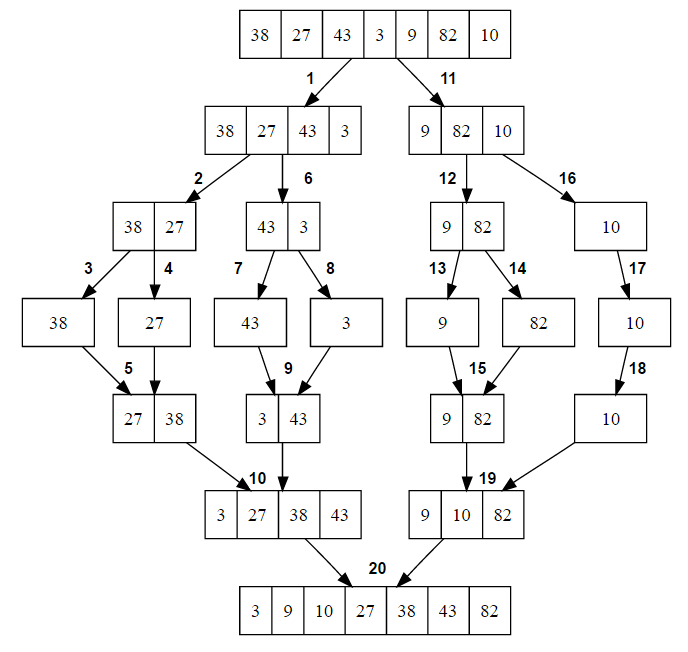
\includegraphics[scale=0.5]{img/mergesort.png}
\end{center}
\medskip\medskip\medskip
La ricorsione “tocca il fondo” quando la sottosequenza ha
lunghezza 1: ogni sequenza di lunghezza 1 è già ordinata.
Fondamentale è l’operazione “combina”, che fonde due
sottosequenze già ordinate: utilizziamo la procedura
\textbf{\texttt{MERGE}($A$, $p$, $q$, $r$)} dove A è un array e $p$, $q$ e $r$ sono indici tali
che $p \leq q \leq r$.
La procedura assume che i sottoarray $A[p..q]$ e $A[q+1..r]$
siano già ordinati e li fonde dando vita a $A[p..r]$.
Ogni sottoarray è ordinato, con i valori più piccoli all’inizio.
Scegliamo il valore più piccolo tra i due valori che stanno
all’inizio dei due array, e lo collochiamo nell’array di output.
Ripetiamo questo passo fino a quando uno dei due
sottoarray non sarà vuoto. Collochiamo dunque tutti i
numeri rimasti nell’altro sottoarray nell’array di output.
Al massimo svolgiamo $n$ passi base, quindi la fusione dei
mazzi impiega un tempo $\Theta(n)$.

\subsection{Procedura \texttt{MERGE}}
\texttt{MERGE}(A, p, q, r)
\begin{lstlisting}[mathescape=true]
n1 = q-p+1
n2 = r-q
crea due nuovi array L[1..n1+1] e R[1..2+1]
for i = 1 to n1
    L[i] = A[p+i-1]
for j=1 to n2
    R[j] =  A[q+j]
L[n1+1] = $\infty$
R[n2+1] = $\infty$
i=1
j=1
for k = p to r
    if L[i] $\leq$ R[j]
          A[k] = L[i]
          i = i+1
    else A[k] = R[j]
          j = j+1
\end{lstlisting}
%
Ovvero:
\begin{lstlisting}
calcola la lunghezza del sottoarray A[p..q]
calcola la lunghezza del sottoarray A[q+1..r]
creiamo gli array R e L (lunghezza n 1 +1 e n 2 +1)

copia il sottoarray A[p..q] in L

copia il sottoarray A[q+1..r] in R
pone il valore sentinella
pone il valore sentinella


combina
\end{lstlisting}
\medskip\medskip
In fondo ai sottoarray $R$ e $L$ mettiamo un valore sentinella ($\infty$): quando incontriamo questo valore in un array,
esso non può essere più piccolo di quello del secondo array. Inoltre sappiamo che quando arriviamo alla
sentinella, tutti i valori precedenti nell’array sono stati posti nell’array di output.

\paragraph{Invariante di ciclo} a ogni iterazione del ciclo for (righe 12-17), il sottoarray $A[p..k]$ contiene ordinati i $k-p$ elementi più piccoli di $L$ e $R$. $L[i]$ e $R[j]$ sono i più piccoli elementi dei propri array che non sono stati copiati in $A$.

\subsubsection{Analisi di \texttt{MERGE}}
\begin{tabularx}{300pt}{X X}
  righe di codice & tempo \\
  \hline
  1 & tempo costante\\
  2 & tempo costante\\
  3 & tempo costante\\
  4 & $n_1$\\
  5 & \\
  6 & $n_2$\\
  7 & \\
  8 & tempo costante\\
  9 & tempo costante\\
  10 & tempo costante\\
  11 & tempo costante\\
  12 & $n$\\
  13 & \\
  14 & \\
  15 & \\
  16 & \\
  17 & \\
\end{tabularx}

\subsection{\texttt{MERGE-SORT}}
Ordina gli elementi nel sottoarray $A[p..r]$. Se $p \geq r$, il sottoarray ha massimo un elemento (è già ordinato),
altrimenti il passo “divide” calcola un indice q che separa $A[p..r]$ in due sottoarray:\medskip\\
\texttt{MERGE-SORT}(A, p, r)
\begin{lstlisting}[mathescape=true]
if p < r
  q = $\lfloor$(p+r)/2$\rfloor$
  $\texttt{MERGE-SORT}$(A, p, q)
  $\texttt{MERGE-SORT}$(A, q+1, r)
  $\texttt{MERGE}$(A, p, q, r)
\end{lstlisting}

\subsection{Analisi degli algoritmi divide et impera}
Quando un algoritmo contiene una chiamata ricorsiva a se stesso, il suo tempo di esecuzione può essere
descritto con un’\textbf{equazione di ricorrenza} (o \textbf{ricorrenza}). Essa esprime il tempo di esecuzione totale di un
problema di dimensione n in funzione del tempo di esecuzione per input più piccoli.
Una ricorrenza per il tempo di esecuzione di un algoritmo divide et impera si basa sui tre passi del paradigma
di base. Supponiamo che n sia la dimensione del problema; $T(n)$ sarà il tempo di esecuzione. Se la dimensione
del problema è sufficientemente piccola, ad esempio $n \leq c$, la soluzione richiede un tempo costante $\Theta(1)$.
Supponiamo che la suddivisione del problema generi a sottoproblemi e che la dimensione di ogni
sottoproblema sia $\frac{1}{b}$ volte la dimensione dell’originale: serve un tempo $T(\frac{n}{b})$ e per $an$ un tempo $aT(\frac{n}{b})$:
\[T(n)= \begin{cases}
          \Theta(1) & se\ n \leq c\\
          aT(\frac{n}{b})+D(n)^*+C(n)^{**} & negli\ altri\ casi
        \end{cases}
\]
* tempo che serve per dividere i problemi in sottoproblemi\\
** tempo che serve per combinare le soluzioni dei sottoproblemi

\subsection{Analisi di \texttt{MERGE-SORT}}
\begin{description}[leftmargin=*]
  \item[Divide] calcola il centro del sottoarray, richiede un tempo costante, $D(n) = \Theta(1)$;
  \item[Impera] risolviamo in modo ricorsivo i due problemi, ognuno di dimensione $\frac{n}{2}$, quindi $2T(\frac{n}{2})$;
  \item[Combina] la procedura \texttt{MERGE} con un sottoarray di n elementi richiede un tempo $\Theta(n)$.
\end{description}
\[T(n)= \begin{cases}
          \Theta(1) & se\ n=1\\
          2T(\frac{n}{2})+\Theta(n)+\Theta(1) & se n > 1
        \end{cases}
\]
\paragraph{Teorema dell'esperto} $T(n)$ è $\Theta(n \lg n)$, dove $\lg$ sta per $\log_2 n$
\medskip\\
\texttt{MERGE-SORT} quindi supera le prestazioni di \texttt{INSERTION-SORT}, il cui tempo di esecuzione è $\Theta(n^2)$, nel caso peggiore.\medskip\\
Possiamo riscrivere la ricorrenza in questo modo:
\[T(n)= \begin{cases}
          c & se\ n=1\\
          2T(\frac{n}{2})+cn & se n > 1
        \end{cases}
\]
$c$ rappresenta il tempo richiesto per risolvere i problemi di dimensione 1, ma anche il tempo dei passi divide e combina per ogni elemento.

\subsection{Albero di ricorsione}
\begin{center}
      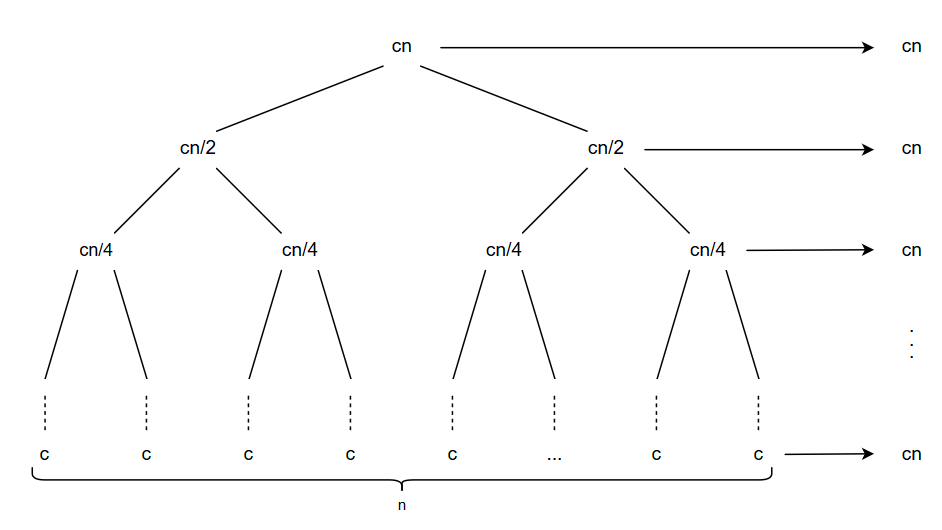
\includegraphics[scale=0.36]{img/alberodiricorsione.png}
\end{center}
Sommiamo i costi per ogni livello dell’albero: il livello i ha $2^i$ nodi, ciascuno dei quali
ha un costo $c(\frac{n}{2^i})$, ogni livello ha dunque un costo totale di $cn$.
Il numero totale di livelli è $\lg n+1$, dove $n$ è il numero delle foglie (uguale alla dimensione dell’input). Il costo totale è di $cn(\lg n +1)$, ovvero $\Theta(n \lg n)$.

\section{\href{https://upload.wikimedia.org/wikipedia/commons/c/c8/Bubble-sort-example-300px.gif}{\texttt{BUBBLESORT}}}
È un noto, ma inefficiente, algoritmo di ordinamento che opera scambiando ripetutamente gli elementi adiacenti che non sono ordinati.\medskip\\
Bubblesort()
\begin{lstlisting}
for i = 1 to A.length-1
  for j = A.length downto i + 1
  	if A[j] < A[j-1]
  		scambia A[j] con A[j-1]
\end{lstlisting}

\section{Efficienza asintotica}
Quando operiamo con dimensioni di input abbastanza grandi da rendere rilevante soltanto il tasso di crescita del tempo di esecuzione, studiamo l’\textbf{efficienza asintotica} degli algoritmi: ci interessa sapere come aumenta il tempo di esecuzione di un algoritmo al crescere della dimensione dell’input al limite. Di solito, un algoritmo che è asintoticamente più efficiente sarà il migliore con tutti gli input, ad eccezione di quelli molto piccoli.

\subsection{Notazione asintotica, funzioni e tempi di esecuzione}
La notazione asintotica si applica alle funzioni. Abbiamo definito il tempo di esecuzione di \texttt{INSERTION-SORT} nel caso peggiore come $\Theta(n^2)$, riferendoci all’equazione $an^2+bn+c$, con $a$, $b$ e $c$ costanti. Scrivendo che il tempo di esecuzione $\Theta(n^2)$ abbiamo trascurato alcuni dettagli.

Una notazione asintotica può anche essere applicata a funzioni che caratterizzano qualche altro aspetto degli algoritmi (quantità di spazio utilizzato) o funzioni che non hanno nulla a che fare con gli algoritmi.

Quando usiamo la notazione asintotica per applicarla al tempo di esecuzione dobbiamo sapere a quale tempo
di esecuzione ci riferiamo. A volte siamo interessati al caso peggiore, a volte vogliamo caratterizzare il tempo indipendentemente da un input.

\subsubsection{Notazione $\Theta$}
Per una funzione $g(n)$, indichiamo con $\Theta(g(n))$ l’insieme delle funzioni
\[\Theta(g(n)) = \{f(n): \exists\ delle\ costanti\ positive\ c_1, c_2\ e\ n_0\ t.c. \]
\[\ 0 \leq c_1g(n) \leq f(n) \leq c_2 g(n) \forall n \geq n_0 \} \]
%
Una funzione $f(n)$ appartiene all’insieme $\Theta(g(n))$ se esistono delle costanti positive $c_1$ e $c_2$ tali che $f(n)$ possa essere racchiusa fra $c_1 g(n)$ e $c_2 g(n)$.
Si dice che $g(n)$ è un \textbf{limite asintoticamente stretto} per $f(n)$.
Ogni membro di $f(n)$ deve essere \textbf{asintoticamente non negativo}, ovvero $f(n)$ deve essere non negativa quando $n$ è sufficientemente grande (una \textbf{funzione asintoticamente positiva} è positiva per qualsiasi valore sufficientemente grande di $n$). Di conseguenza anche $g(n)$ deve essere asintoticamente non negativa.
\begin{center}
      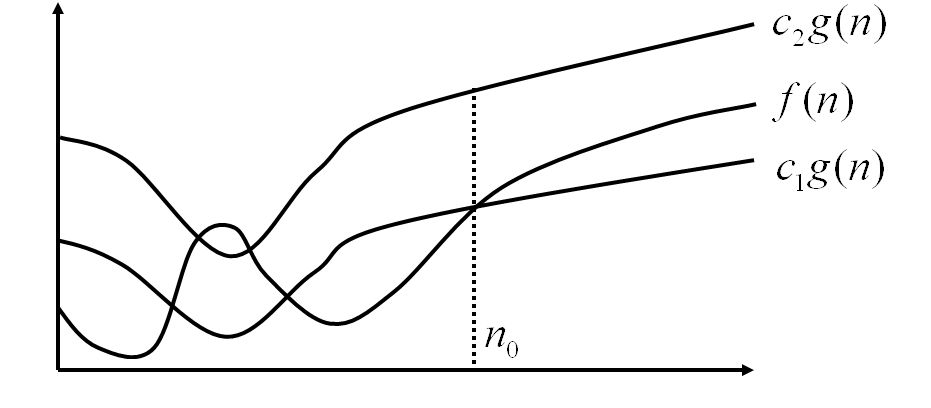
\includegraphics[scale=0.4]{img/teta.png}
\end{center}
Informalmente, per trovare una notazione $\Theta$, possiamo escludere i termini di ordine inferiore e ignorare il coefficiente del termine di ordine più elevato.

\subsubsection{Notazione $O$}
\[O(g(n)) = \{f(n): \exists \ delle\ costanti\ positive\ c\ e\ n_0\ t.c.\]
\[0 \leq f(n) \leq cg(n) \forall n \geq n_0 \}\]
La notazione $\Theta$ limita asintoticamente una funzione da sopra e da sotto. Quando abbiamo soltanto un \textbf{limite asintotico superiore}, utilizziamo una notazione $O$. Per qualsiasi valore $n$ a destra di $n_0$, il valore di $f(n)$ coincide o sta sotto $cg(n)$.
\begin{center}
      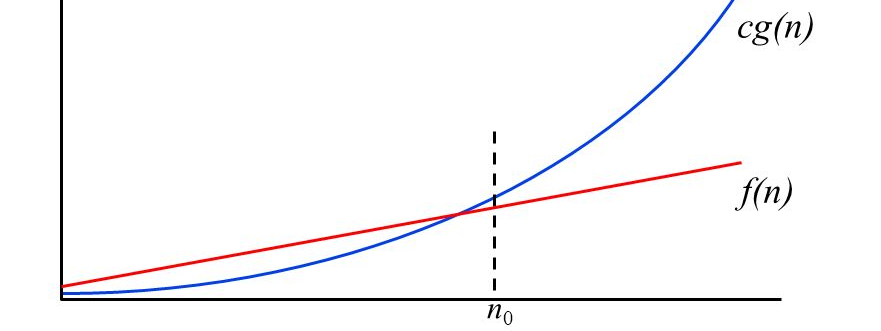
\includegraphics[scale=0.4]{img/ogrande.png}
\end{center}
Si dice che $f(n)$ è $O$ di $cg(n)$.

\subsubsection{Notazione $\Omega$}
Fornisce un \textbf{limite asintotico inferiore}.
\[\Omega (g(n)) = \{f(n): \exists \ delle\ costanti\ positive\ c\ e\ n_0\ t.c.\]
\[0 \leq cg(n) \leq f(n) \forall n \geq n_0 \} \]
Per qualsiasi valore $n$ a destra di $n_0$ , il valore di $f(n)$ coincide o sta sopra $cg(n)$.
\begin{center}
      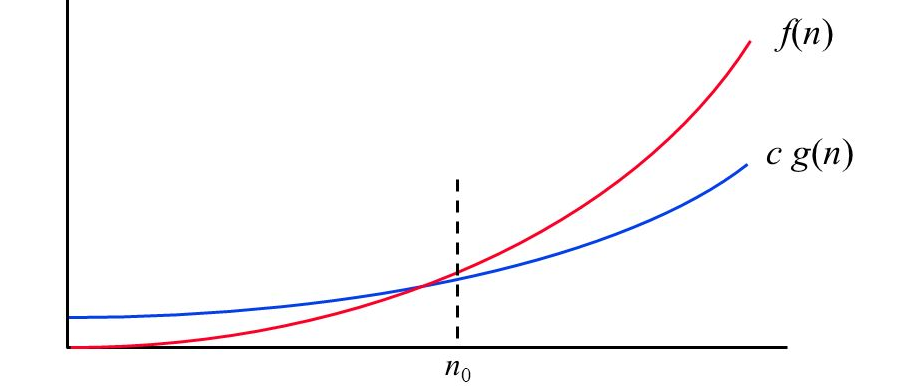
\includegraphics[scale=0.4]{img/omega.png}
\end{center}
Si dice che $f(n)$ è $\Omega$ di $cg(n)$.

\paragraph{Teorema} Per ogni coppia di fuzioni $f(n)$ e $g(n)$, si ha $f(n)$ = $\Theta(g(n))$ se e solo se $f(n) = O(g(n)) e f(n) = \Omega (g(n))$.

\subsubsection{Notazione asintotica nelle equazioni e nelle disequazioni}
Quando una notazione asintotica appare in una formula, essa va trattata come se indicasse una funzione
anonima, di cui non è importante fare il nome. In questo modo è possibilie eliminare i dettagli superflui e ingombranti da un’equazione.
Il numero di funzioni anonime in un’espressione è sottinteso che sia uguale al numero di volte che appare la notazione asintotica; per esempio, in $\sum_{i=1}^n O(i)$ c’è una sola funzione anonima (una funzione di i). Questa espressione quindi è diversa da $O(1)+O(2)+...+O(n)$.
In alcuni casi la notazione asintotica si trova sul lato sinistro dell’equazione, ad esempio in $2n^2+\Theta(n) =\Theta(n^2)$.
Per qualsiasi funzione $f(n) \in \Theta(n)$, c’è qualche funzione $g(n) \in \Theta(n^2)$ t.c. $2n^2 +f(n) = g(n)$ per ogni $n$.
Il lato destro di un’equazione fornisce un livello di dettaglio più grossolano del lato sinistro.

\subsubsection{Notazione $o$}
Il limite asintotico superiore ($=$) può essere stretto oppure no.
$2n^2 = O(n^2)$ è asintoticamente stretto
$2n = O(n^2)$ non è asintoticamente stretto. Questo lo definiamo con $o$.
In $O$, il limite vale per qualche costante $c > 0$; in $o$, il limite vale per tutte le costanti $c > 0$.

\subsubsection{Notazione $\omega$}
Analogamente, $\omega$ sta a $\Omega$ come $o$ sta a $O$.
Usiamo la notazione $\omega$ per indicare un limite non asintoticamente stretto.

\subsubsection{Confronto di funzioni}
\begin{tabularx}{400pt}{l X}
  \multirow{5}{*}{Proprietà transitiva} & $f(n) = \Theta(g(n)) e g(n) = \Theta(h(n)) \Rightarrow f(n) = \Theta(h(n))$\\
  & $f(n) = O(g(n)) e g(n) = O(h(n)) \Rightarrow f(n) = O(h(n))$\\
  & $f(n) = o(g(n)) e g(n) = o(h(n)) \Rightarrow f(n) = o(h(n))$\\
  & $f(n) = \Omega(g(n)) e g(n) = \Omega(h(n)) \Rightarrow f(n) = \Omega(h(n))$\\
  & $f(n) = \omega(g(n)) e g(n) = \omega(h(n)) \Rightarrow f(n) = \omega(h(n))$\\
  \hline
  \multirow{3}{*}{Proprietà riflessiva} & $f(n) = \Theta(f(n))$\\
  & $f(n) = O(f(n))$\\
  & $f(n) = \Omega(f(n))$\\
  \hline
  Proprietà simmetrica & $f(n) = \Theta(g(n)) \Leftrightarrow g(n) = \Theta(f(n))$\\
  \hline
  \multirow{2}{*}{Simmetria trasposta} & $f(n) = O(g(n)) \Leftrightarrow g(n) = \Omega(f(n))$\\
  & $f(n) = o(g(n)) \Leftrightarrow g(n) = \omega(f(n))$\\
  \hline
  Tricotomia & Se $a$ e $b$ sono due numeri reali qualsiasi deve valare solo una delle seguenti relazioni:
$a < b$, $a = b$, $a > b$
\end{tabularx}

\subsubsection{Funzioni monotòne}
\begin{tabular}{l l}
monotona crescente & $m \leq n \Rightarrow f(m) \leq f(n)$\\
monotona decrescente & $m \leq n \Rightarrow f(m) \geq f(n)$\\
strettamente crescente & $m < n \Rightarrow f(m) < f(n)$\\
strettamente decrescente & $m < n \Rightarrow f(m) > f(n)$
\end{tabular}

\subsection{Altro}
\subsubsection{Floor e ceiling}
\begin{tabular}{l l l}
Floor & $\lfloor ... \rfloor$ & difetto\\
Ceiling & $\lceil ... \rceil$ & eccesso
\end{tabular}

\section{Ricorrenze}
Una ricorrenza è un’equazione o disequazione che descrive una funzione in termini del suo valore con input
più piccoli. Abbiamo diversi metodi per risolvere le ricorrenze (cioè per ottenere dei limiti asintotici “$\Theta$” o “$O$”):
\begin{itemize}
  \item \textbf{Metodo della sostituzione}: ipotizziamo un limite e usiamo l’induzione matematica per dimostrare che la nostra ipotesi è corretta.
  \item \textbf{Metodo dell’albero della ricorsione}: converte la ricorrenza in un albero i cui nodi rappresentano i costi ai vari livelli della ricorsione.
  \item \textbf{Metodo dell’esperto}: fornisce i limiti per ricorrenze nella forma $T(n) = aT(\frac{n}{b}) + f(n)$ dove $a\geq1$, $b>1$ e $f(n)$ è una funzione data. Una ricorrenza come questa caratterizza un algoritmo che crea a sottoproblemi, ciascuno di dimensione $\frac{1}{b}$ e in cui i passi divide e combina insieme richiedono un tempo $f(n)$.
\end{itemize}

\subsection{Dettagli tecnici}
Quando definiamo e risolviamo le ricorrenze, trascuriamo alcuni dettagli tecnici. Ad esempio, se chiamiamo
\texttt{MERGE-SORT} su $n$ elementi con $n$ dispari, avremo sottoproblemi di dimensione $\lfloor\frac{n}{2}\rfloor$ e $\lceil \frac{n}{2} \rceil$. La ricorrenza è effettivamente
\[T(n)= \begin{cases}
          \Theta(1) & se\ n=1\\
          T(\lceil \frac{n}{2} \rceil) + T(\lfloor \frac{n}{2} \rfloor) + \Theta(n) & se n > 1
        \end{cases}
\]
%
Solitamente però omettiamo le condizioni al contorno e le operazioni di floor e ceiling: a noi interessa infatti il tasso di crescita, che rimane immutato e non dipende da fattori costanti.

\subsection{Il metodo di sostituzione per risolvere le ricorrenze}
\begin{itemize}
  \item Ipotizzare la forma della soluzione
  \item Usare l’induzione matematica per trovare le costanti e dimostrare che la soluzione funziona
\end{itemize}
%
Questo metodo può essere utilizzato per determinare il limite superiore o inferiore di una ricorrenza.
Ad esempio determiniamo il limite superiore per la ricorrenza $T(n) = 2T(\lfloor \frac{n}{2} \rfloor) + n$.
Supponiamo che la soluzione sia $T(n) = O(n \lg n)$.
Il metodo consiste nel dimostrare che $T(n) \leq cn \lg n$ per una scelta appropriata della costante $c > 0$.
Supponiamo che questo limite sia valido per $\lfloor\frac{n}{2}\rfloor$, ovvero che $T(\lfloor \frac{n}{2} \rfloor) \leq c\lfloor \frac{n}{2} \rfloor lg ( \lfloor \frac{n}{2} \rfloor )$.\medskip\\
Avremo:
\[T(n) \leq 2(c\lfloor \frac{n}{2} \rfloor \lg ( \lfloor \frac{n}{2} \rfloor ) ) + n \]
\[\leq cn \lg (\frac{n}{2}) + n \]
\[= cn \lg n - cn \lg 2 + n \]
\[= cn \lg n - cn + n \]
\[\leq cn \lg n \]
L’ultimo passo è vero quando $c \geq 1$.
Dobbiamo ora dimostrare che la nostra soluzione vale per le condizioni al contorno.
Dobbiamo dimostrare che è possibile scegliere una costante c sufficientemente grande in modo che il limite
$T(n) \leq cn \lg n$ sia valido anche per le condizioni al contorno. Sfruttiamo la notazione asintotica che ci richiededi provare che $T(n) \leq cn \lg n$ per $n > n_0$ dove $n_0$ è una costante arbitrariamente scelta. In questo caso è
sufficiente scegliere $c \geq 2$.

\subsubsection{Formulare una buona ipotesi}
Se una ricorrenza è simile a una già vista, ha senso provare una soluzione analoga.
Ad esempio, prendiamo $T(n) = 2T(\lfloor \frac{n}{2} \rfloor + 17 ) + n$.
Il termine aggiuntivo 17 non influisce in modo sostanziale alla soluzione della ricorrenza. Quando $n$ è grande,
la differenza tra $T(n) = 2T(\lfloor \frac{n}{2} \rfloor + 17 ) + n$ e $T(n) = 2T(\lfloor \frac{n}{2} \rfloor) + n$ non è così grande: $n$ viene diviso circa
a metà in entrambi i casi.
Un altro metodo è quello di dimostrare dei limiti superiori e inferiori laschi (non stretti) per la ricorrenza e poi
ridurre man a mano il grado di incertezza.

\subsubsection{Finezze}
Ci sono casi in cui, pur avendo ipotizzato correttamente un limite asintotico per la soluzione della ricorrenza, i conti non tornano. Spesso ciò accade perché l’ipotesi induttiva non è abbastanza forte per dimostrare il limite esatto. A volte basta correggere l’ipotesi sottraendo un termine di ordine inferiore.

\subsubsection{Sostituzione di variabili}
\[T(n) = 2T(\lfloor\sqrt{n}\rfloor) + \lg n\]
Poniamo $m = \lg n$
\[T(2^m) = 2T(2^{\frac{m}{2}}) + m\]
Poniamo $S(m) = T(2^m)$
\[S(m) = 2S(\frac{m}{2}) + m\]
che ha soluzione
\[S(m) = O(m \lg m)\]
Ripristinando $T$, otteniamo \[T(n) = O(m \lg m) = O(\lg n \lg (\lg n))\]

\subsection{Il metodo dell’albero di ricorsione per risolvere le ricorrenze}
In un albero di ricorsione ogni nodo rappresenta il costo di un singolo sottoproblema. Sommiamo i costi
all’interno di ogni livello per avere un insieme di costi per livello, poi sommiamo tutti i costi per livello per
ottenere il costo totale.
Un albero è un ottimo metodo per avere un’ipotesi, che poi verrà verificata con il metodo di sostituzione (ma
possiamo anche usarlo come prova diretta di una soluzione di ricorrenza).

\subsubsection{Esempio}
Sia data la ricorrenza $T(n) = 3T(\lfloor \frac{n}{4} \rfloor) + \Theta (n^2)$
Iniziamo cercando un limite superiore per la soluzione.
Sappiamo che \emph{floor} e \emph{ceiling} non influiscono sulla risoluzione delle ricorrenze; creiamo
un albero di ricorsione per la ricorrenza $T(n) = 3T(\lfloor \frac{n}{4} \rfloor) + cn^2$ , ricordando che $c$ è
costante.
\begin{center}
      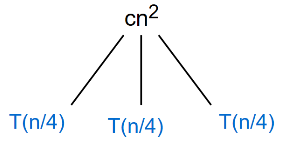
\includegraphics[scale=0.5]{img/alberoricorrenze1.png}
\end{center}
Le dimensioni dei sottoproblemi
diminuiscono di un fattore 4 ogni volta che
scendiamo di livello. Alla fine dovemmo
giungere a una condizione al contorno.
La dimensione del sottoproblema per un
nodo è alla profondità $i$ è $\frac{n}{4}^i$ . La
dimensione del sottoproblema diventa
quindi $n=1$ quando $\frac{n}{4}^i =1$ ovvero quando $i
= \log_4 n$.
L’albero ha $log_4 n +1$ livelli.
Determiniamo ora il costo a ogni livello
dell’albero. Ogni livello ha 3 volte i nodi del
livello precedente, quindi il numero di nodi
alla profondità $i$ è $3^i$ . Poiché le dimensioni di
un sottoproblema diminuiscono di 4 volte ogni volta, ogni nodo alla profondità $i$ ha un costo di $c(\frac{n}{4}^i)^2$ . Il costo
totale di tutti i nodi alla profondità i è $(\frac{3}{16})^i cn^2$ . Nell’ultimo livello ogni nodo ha costo $T(1)$, per un costo totale
di $n^{\log_4 3} T(1)$, che è $\Theta n^{\log_4 3}$ , perché supponiamo che $T(1)$ sia una costante.
Sommiamo ora il costo di tutti i livelli. La formula si presenta complicata. Possiamo però approssimare ancora
e usare come limite superiore una serie geometrica decrescente infinita.
\begin{center}
      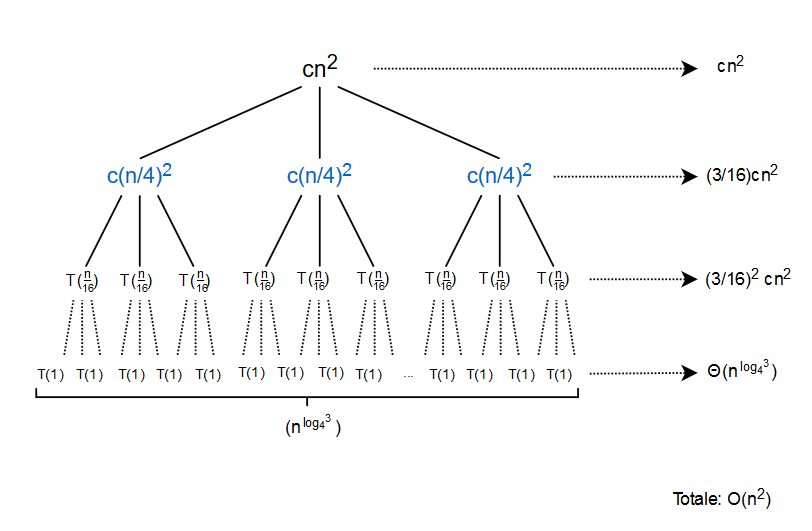
\includegraphics[scale=0.4]{img/alberoricorrenze2.png}
\end{center}
Il costo totale dell’albero è dominato dal costo della radice.
Possiamo ora usare il metodo di sostituzione per dimostrare che la nostra ipotesi era corretta, ovvero
$T(n)=O(n^2)$ è un limite superiore per la ricorrenza $T(n) = 3T(\lfloor \frac{n}{4} \rfloor) + \Theta (n^2)$.
Dobbiamo dimostrare che $T(n) \leq dn^2$ per qualche costante $d > 0$.
Otteniamo:
\[T(n) \leq 3T(\lfloor \frac{n}{4} \rfloor) + c n^2\]
\[\leq 3d\lfloor \frac{n}{4} \rfloor^2 + c n^2\]
\[\leq 3d (\frac{n}{4})^2 + c n^2\]
\[= \frac{3}{16} d n^2 + c n^2\]
\[\leq d n^2\]
L’ultimo passaggio è vero quando $d \geq (\frac{16}{13})c$.

\subsection{Il metodo del’esperto per risolvere le ricorrenze}
Si usa per risolvere ricorrenze della forma $T(n) = aT(\frac{n}{b})+f(n)$, dove $a \geq 1$ e $b > 1$ sono costanti e $f(n)$ è
asintoticamente positiva.
Questa ricorrenza descrive il tempo di esecuzione di un algoritmo che divide un problema di dimensione n in
a sottoproblemi, ciascuno di dimensione $\frac{n}{b}$. I sottoproblemi vengono risolti in modo ricorsivo, ciascuno nel
tempo $T(\frac{n}{b})$.

\paragraph{Teorema} date le costanti $a \geq 1$ e $b > 1$ e la sua funzione $f(n)$, sia $T(n)$ una funzione definita sufli interi non
negativi della ricorrenza $T(n) = aT(\frac{n}{b})+f(n)$ dove $\frac{n}{b}$ rappresenta $\lfloor\frac{n}{b}\rfloor$ o $\lceil\frac{n}{b}\rceil$. Allora $T(n)$ può essere
asintoticamente limitata nei seguenti modi:
\begin{enumerate}
  \item se $f(n) = O(n^{\log_b a-\epsilon})$ per qualche costante $\epsilon > 0$, allora $T(n) = \Theta(n^{\log_b a})$
  \item se $f(n) = \Theta(n^{\log_b a})$, allora $T(n) = \Theta(n^{\log_b a} \lg n)$
  \item se $f(n) = \Omega(n^{\log_b a + \epsilon} )$ per qualche costante $\epsilon > 0$ e se $af(\frac{n}{b}) \leq cf(n)$ per qualche costante $c < 1$ e per ogni $n$
sufficientemente grande, allora $T(n) = \Theta(f(n))$.
\end{enumerate}
Nel primo caso $f(n)$ deve essere polinomialmente più piccola di $n^{\log_b a}$ , ovvero $f(n)$ deve essere
asintoticamente più piccola di $n^{\log_b a}$ per un fattore $n^\epsilon$ per qualche costante $\epsilon > 0$.
Nel terzo caso $f(n)$ deve essere polinomialmente più grande grande di $n^{\log_b a}$ , e soddisfare le condizioni di
regolarità $af(\frac{n}{b}) \leq cf(n)$.

I tre casi non coprono tutte le funzioni possibili di $f(n)$.

\subsubsection{Applicazione del metodo dell’esperto}
Determiniamo quale caso del teorema dell’esperto possiamo applicare (se esiste) e scriviamo la soluzione

\section{Heap}
Un heap (binario) è una struttura dati composta da un array che possiamo considerare come un albero binario
quasi completo. Ogni nodo è un elemento dell’array. Tutti i livelli sono riempiti, tranne eventualmente l’ultimo
che da sinistra è riempito fino ad un certo punto.
Anche se ci sono numeri memorizzati in tutto l’array, solo quelli $A[1 .. A.heap-size]$ sono validi nell’heap. La
radice dell’albero è $A[1]$.\medskip\\
%
Se $i$ è l’indice di un nodo possiamo calcolare gli indici di:
\begin{itemize}[leftmargin=*]
\item \texttt{PARENT}($i$) padre
\begin{lstlisting}[mathescape=true]
return $\lfloor i/2 \rfloor$
\end{lstlisting}
Può calcolare $\lfloor i/2 \rfloor$ con uno scorrimento di una posizione a destra della rappresentazione di $i$.
\item \texttt{LEFT}($i$) figlio sx
\begin{lstlisting}[mathescape=true]
return 2i
\end{lstlisting}
La procedura può calcolare 2i con una sola istruzione, facendo scorrere di una
posizione a sinistra la rappresentazione binaria di i.
\item \texttt{RIGHT}($i$) figlio dx
\begin{lstlisting}[mathescape=true]
return 2i+1
\end{lstlisting}
La procedura può calcolare 2i+1 facendo scorrere di una posizione a sinistra la
rappresentazione binaria di i e aggiungendo 1 come bit meno significativo.
\end{itemize}

\paragraph{altezza di un nodo} numero di archi nel cammino semplice più lungo che dal nodo scende fino a una foglia.
\paragraph{altezza di un heap} altezza della radice. Poiché un heap di n elementi è basato su un albero binario completo, la sua altezza
è $\Theta(\lg n)$.

\subsection{Max-heap e Min-heap}
Gli heap binari si dividono in
\begin{description}[leftmargin=*]
  \item[max-heap] per ogni nodo diverso dalla radice si ha $A[\texttt{PARENT}(i) \geq A[i]$. Il valore di un nodo è al
massimo quello di suo padre. L’elemento più grande è memorizzato nella radice.
  \item[min-heap] per ogni nodo diverso dalla radice si ha $A[\texttt{PARENT}(i) \leq A[i]$. Il più piccolo elemento
è nella radice.
\end{description}

\subsection{Conservare la proprietà dell’heap}
Useremo la procedura \texttt{MAX-HEAPIFY} . I suoi input sono un array A e un indice i.
Quando viene chiamata, assume che gli alberi binari con radici in $\texttt{LEFT}(i)$ e $\texttt{RIGHT}(i)$ siano max-heap, ma che
$A[i]$ possa essere più piccolo dei suoi figli (violando la proprietà del max-heap).
La procedura fa scendere il valore $A[i]$ nel max-heap in modo che il sottoalbero con radice di indice i diventi
un max-heap: a ogni passo, tra gli elementi $A[i]$, $A[\texttt{LEFT}(i)]$ e $A[\texttt{RIGHT}(i)]$ viene determinato il più grande. Il
suo indice viene memorizzato in \emph{massimo}. Se $A[i]$ è più grande, il sottoalbero con radice $i$ è un max-heap e la
procedura termina. Altrimenti, uno dei due figli ha l’elemento più grande e viene scambiato $A[i]$ con
$A[massimo]$; il sottoalbero però potrebbe violare la proprietà del max-heap; viene chiamata ricorsivamente la
subroutine \texttt{MAX-HEAPIFY}.\medskip\medskip\\
\texttt{MAX-HEAPIFY}$(A, i)$
\begin{lstlisting}[mathescape=true]
l = $\texttt{LEFT}(i)$
r = $\texttt{RIGHT}(i)$
if l $\leq$ A.heap-size and $A[l] > A[i]$
     massimo = l
else massimo = i
if r $\leq$ A.heap-size and $A[r] > A[massimo]$
     massimo = r
if massimo $\neq$ i
     scambia A[i] con A[]
     $\texttt{MAX-HEAPIFY}(A, massimo)$
\end{lstlisting}
Il tempo di esecuzione di \texttt{MAX-HEAPIFY} in un sottoalbero di dimensione $n$ con radice in un nodo i è pari al
tempo $\Theta(1)$ per sistemare le relazioni fra gli elementi $A[i]$, $A[ \texttt{LEFT} (i)]$ e $A[ \texttt{RIGHT} (i)]$, più il tempo per eseguire
MAX-HEAPIFY in un sottoalbero con radice in uno dei figli del nodo $i$.
La dimensione dei sottoalberi dei figli non supera $2\frac{n}{3}$.
Il tempo di esecuzione può essere descritto dalla ricorrenza $T(n) \leq T(2\frac{n}{3}) + \Theta(1)$. La soluzione è $T(n) = O(\lg n)$,
oppure $O(h)$ (nodo di altezza $h$).

\subsection{Costruire un heap}
Possiamo utilizzare la procedura \texttt{MAX-HEAPIFY} dal basso verso l’alto per convertire un array in un max-heap.
La procedura \texttt{BUILD-MAX-HEAP} attraversa i restanti nodi dell’albero ed esegue \texttt{MAX-HEAPIFY} in ciascuno di
essi.\medskip\medskip\\
\texttt{BUILD-MAX-HEAP}$(A)$
\begin{lstlisting}[mathescape=true]
A.heap-size = A.length
for $i = \lfloor A.length/2 \rfloor$ downto 1
$\texttt{MAX-HEAPIFY} (A, i)$
\end{lstlisting}

\paragraph{Invariante di ciclo} all’inizio di ogni ciclo for, ogni nodo i+1, i+2, ..., n è la radice
di un heap\medskip\\
%
Possiamo calcolare un semplice limite superiore sul tempo di esecuzione di \texttt{BUILD-MAX-HEAP} nel seguente
modo: ogni chiamata di \texttt{MAX-HEAPIFY} costa un tempo $O(\lg n)$ e ci sono $O(n)$ di queste chiamate, per un totale
di $O(n \lg n)$. Questo limite però non è asintoticamente stretto.
Osserviamo che il tempo per eseguire \texttt{MAX-HEAPIFY} in un nodo varia con l’altezza del nodo dell’albero. Un
heap di n elementi ha un’altezza $\lfloor\lg n\rfloor$ e per ogni $h$, al massimo $\lceil \frac{n}{2}^{h+1} \rceil$ nodi di altezza $h$. Il tempo richiesto
dalla procedura quando viene chiamata per un nodo di altezza h è $O(h)$, quindi il costo totale di \texttt{BUILD-MAX-HEAP} è limitato superiormente da
\[\sum^{\lfloor \lg n \rfloor}_{h=0} \lceil \frac{n}{2^{h+1}} \rceil O(h) = O (n \sum^{\lfloor \lg n \rfloor}_{h=0} \frac{h}{2^h}) = O (n \sum^\infty_{h=0} \frac{h}{2^h}) = O(n)\]
%
Possiamo costruire un min-heap utilizzando la procedura \texttt{BUILD-MIN-HEAP}, che è uguale a \texttt{BUILD-MAX-
HEAP}, ma la chiamata di \texttt{MAX-HEAPIFY} alla riga 3 è sostituita dalla chiamata di \texttt{MIN-HEAPIFY}.

\subsection{L’algoritmo \href{https://cdn-images-1.medium.com/max/1600/1*LVcbTeL6zPLfDHiQ2w3Jtw.gif}{\texttt{HEAPSORT}}}
Inizia costruendo con \texttt{BUILD-MAX-HEAP} un max-heap nell’array di input $A[1..n]$ $(n=A.length)$. L’elemento più
grande è memorizzato nella radice $A[1]$, può essere scambiato con A[n] per andare nella sua posizione finale
corretta. “Togliamo” il nodo n dall’heap: $A[n-1]$ può essere facilmente trasformato in un max-heap. I figli della
radice sono un max-heap, ma la nuova radice potrebbe violare la proprietà del max-heap. Per ripristinare la
proprietà chiamiamo di \texttt{MAX-HEAPIFY}$(A, 1)$. Esso lascia un max-heap in $A[1.. (n-1)]$. L’algoritmo viene ripetuto
per il max-heap di dimensione $n-1$ e così via fino a un heap di dimensione 2.\medskip\medskip\\
%
\texttt{HEAPSORT}$(A)$
\begin{lstlisting}[mathescape=true]
$\texttt{BUILD-MAX-HEAP}(A)$
for i = A.length downto 2
scambia A[1] con A[i]
A.heap-size = A.heap-size-1
$\texttt{MAX-HEAPIFY}(A, 1)$
\end{lstlisting}

\subsection{Code di priorità}
Una buona implementazione di quicksort solitamente batte heapsort. Tuttavia la struttura dati heap ha
molteplici usi, ad esempio le \textbf{code di priorità}.
Una coda di priorità è una struttura dati che serve a mantenere un insieme S di elementi ognuno dei quali ha
un valore associato detto \textbf{chiave}.
%
\begin{center}
      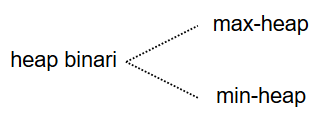
\includegraphics[scale=0.4]{img/codepriorita.png}
\end{center}
%
Una coda di max-priorità supporta le operazioni:
\begin{itemize}[leftmargin=*]
  \item \texttt{INSERT}$(S, x)$ - Inserisce x nell’insieme S
  \item \texttt{MAXIMUM}$(S)$ - Restituisce l’elemento di S con la chiave più grande
  \item \texttt{EXTRACT-MAX}$(S)$ - Rimuove e restituisce l’elemento di S con la chiave più grande
  \item \texttt{INCREASE-KEY}$(S, x, k)$ - Aumenta il valore della chiave dell’elemento x al nuovo valore k, che si suppone sia almeno grande quantoil valore corrente della chiave dell’elemento x
\end{itemize}

La coda di max-priority tiene traccia dei lavori da svolgere e delle loro relative proprietà. Quando un lavoro è
ultimato o interrotto, lo scheduler seleziona il lavoro con priorità più alta fra quelli in attesa, chiamando
\texttt{EXTRACT-MAX}. In ogni momento si può inserire un lavoro tramite INSERT .
Una coda di min-priority supporta le operazioni \texttt{INSERT}, \texttt{MAXIMUM}, \texttt{EXTRACT-MIN}, \texttt{DECREASE-KEY}.


Quando un heap viene utilizzato per implementare una coda di priorità, spesso occorre memorizzare in ogni
elemento dell’heap un \textbf{handle} (aggancio) al corrispondente oggetto dell’applicazione. Tipicamente l’handle è un indice dell’array.
\begin{itemize}[leftmargin=*]
  \item
\texttt{HEAP-MAXIMUM}$(A)$
\begin{lstlisting}[mathescape=true]
return $A[1]$
\end{lstlisting}

  \item
  \texttt{HEAP-EXTRACT-MAX}$(A)$
\begin{lstlisting}[mathescape=true]
if A.heap-size < 1
    error "underflow dell'heap"
max = A[1]
A[1] = A[A.heap-size]
A.heap-size = A.heap-size -1
$\texttt{MAX-HEAPIFY}(A, 1)$
return max
\end{lstlisting}
Il tempo di esecuzione è $O(\lg n)$.

  \item
\texttt{HEAP-INCREASE-KEY}$(A, i, key)$
\begin{lstlisting}[mathescape=true]
if key < A[i]
    error "nuova chiave piu' piccola di quella corrente"
A[i] = key
while i > 1 and $A[\texttt{PARENT}(i)] < A[i] ]$
    scambia $A[i]$ con $A[\texttt{PARENT}(i)]$
    $i = \texttt{PARENT}(i)$
\end{lstlisting}
Il tempo di esecuzione con un heap di
n elementi è $O(\lg n)$.

  \item
\texttt{MAX-HEAP-INSERT}$(A, key)$
\begin{lstlisting}[mathescape=true]
A.heap-size = A.heap-size +1
A[A.heap-size] = $- \infty$
$\texttt{HEAP-INCREASE-KEY}(A, A.heap-size, key)$
\end{lstlisting}
Il tempo di esecuzione con un heap di
n elementi è $O(\lg n)$.
\end{itemize}

\section{\href{https://upload.wikimedia.org/wikipedia/commons/9/9c/Quicksort-example.gif}{\texttt{QUICKSORT}}}
Quicksort è un algoritmo di ordinamento ricorsivo in place non stabile.
Appartiene alla classe degli algoritmi divide et impera, dal momento che
scompone ricorsivamente i dati da processare in sottoprocessi.
\begin{description}[leftmargin=*]
  \item[divide] partiziona l’array $A[p..r]$ in due sottoarray $A[p..q-1]$ e $A[q+1..r]$
  tali che ogni elemento di $A[p..q-1]$ sia minore o uguale ad $A[q]$ che, a sua
  volta è minore o uguale a ogni elemento di $A[q+1..r]$
  \item[impera] ordina i due sottoarray chiamando ricorsivamente quicksort
  \item[combina] poiché i sottoarray sono già ordinati, non occorre alcun
  lavoro per combinarli
\end{description}
\begin{center}
      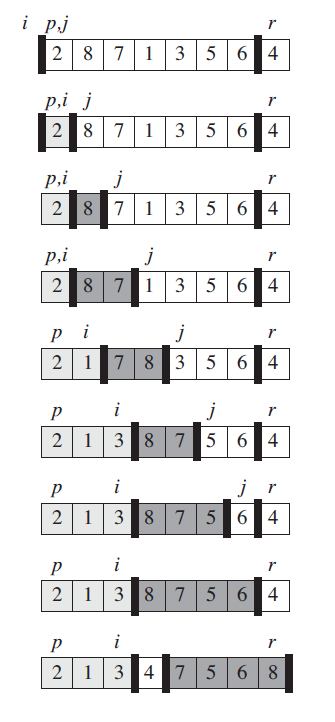
\includegraphics[scale=0.5]{img/quicksort.png}
\end{center}
Tale procedura ricorsiva viene comunemente detta \texttt{PARTITION}: preso un
elemento chiamato \textbf{pivot} da una struttura dati (es. array) si pongono gli
elementi minori a sinistra rispetto al pivot e gli elementi maggiori a destra.
L'operazione viene quindi reiterata sui due insiemi risultanti fino al
completo ordinamento della struttura.
Il \texttt{QUICKSORT} è l'algoritmo di ordinamento che ha, nel caso medio,
prestazioni migliori tra quelli basati su confronto.\medskip\\
\texttt{QUICKSORT}$(A, p, r)$
\begin{lstlisting}[mathescape=true]
if p < r
    $q = \texttt{PARTITION}(A, p, r)$
    $\texttt{QUICKSORT}(A, p, q-1)$
    $\texttt{QUICKSORT}(A, q+1, r)$
\end{lstlisting}

\subsection{Partizionare l’array}
L’elemento chiave è la procedura \texttt{PARTITION}, che riarrangia il sottoarray $A[p..r]$ sul posto.
\texttt{PARTITION}$(A, p, r)$
\begin{lstlisting}[mathescape=true]
x = A[r]
i = p-1
for j = p to r-1
    if $A[j] \leq x$
        i = i+1
        scambia A[i] con A[j]
scambia A[i+1] con A[r]
return i+1
\end{lstlisting}
\medskip
Ovvero:\\
seleziona un elemento come pivot intorno al quale partizionare l’array\\
All’inizio di ogni iterazione del ciclo for, per qualsiasi indice k dell’array:\\
1. se $p \leq k \leq i$, allora $A[k] \leq x$\\
2. se $i+1 \leq k \leq j-1$, allora $A[k] > x$\\
3. se $k = r$, allora $A[k] = x$\\
Inserisce il pivot al suo posto in mezzo all’array, scambiandolo con\\
l’elemento più a sx che è $> x$ e restituisce il nuovo indice del pivot.

\paragraph{Invariante di ciclo}
\begin{description}[leftmargin=*, noitemsep]
  \item[inizializzazione] prima della prima iterazione del ciclo, $i = p-1$ e $j = p$.
  \item[conservazione] quando $A[j] > x$, viene incrementata $j$. Quando $A[j] \leq x$, viene incrementato $i$ e scambiati $A[i]$ e
$A[j]$, poi viene incrementato $j$.
  \item[conclusione] alla fine del ciclo, $j = r$.
\end{description}
%
Il tempo di esecuzione di \texttt{PARTITION} con il sottoarray $A[p..r]$ è $\Theta(n)$, dove $n = r-p+1$.

\subsection{Prestazioni di \texttt{QUICKSORT}}
Il tempo di esecuzione di \texttt{QUICKSORT} dipende dal fatto che il partizionamento può essere bilanciato o meno, e
questo a sua volta dipende da quali elementi vengono utilizzati per il partizionamento. Se esso è bilanciato,
l’algoritmo ha la stessa velocità asintotica di merge-sort. Se è sbilanciao, può essere asintoticamente lento
come \texttt{INSERTION-SORT}.

\subsubsection{Partizionamento nel caso peggiore}
Il comportamento nel caso peggiore si verifica quando il partizionamento produce un sottoproblema con $n-1$
elementi e uno con 0 elementi. Se questo sbilanciamento si verifica in ogni chiamata ricorsiva, poiché per una
chiamata ricorsiva su un array vuoto $T(0) = \Theta(1)$, la ricorrenza può essere espressa così:
\[T(n) = T(n-1) + T(0) + \Theta(n)\]
\[= T(n-1) + \Theta(n)\]
Se sommiamo i costi a ogni livello della ricorsione, otteniamo una serie aritmetica di valore $+ \Theta(n^2)$.
Il tempo di esecuzione $\Theta(n^2)$ si ha quando l’array di input è già completamente ordinato, situazione in cui
insertion-sort è eseguito nel tempo $O(n)$.

\subsubsection{Partizionamento nel caso migliore}
Nel caso di bilanciamento massimo, vengono prodotti due sottoproblemi, ciasuno di dimensione non maggiore
di $\frac{n}{2}$ (uno ha dimensione $\lfloor \frac{n}{2} \rfloor$ e l’altro $\lceil \frac{n}{2} \rceil -1)$. In questo caso viene eseguito molto più velocemente. La
ricorrenza è:
\[T(n) \leq 2T(\frac{n}{2}) + \Theta(n)\]
che ha soluzione $T(n) = O(n \lg n)$.

\subsubsection{Partizionamento bilanciato}
Il tempo di esecuzione di quicksort nel caso medio è vicino al caso migliore.
Supponiamo una ripartizione 9 a 1, che potrebbe sembrare molto sbilanciata. Otteniamo la ricorrenza:
\[T(n) = T(\frac{9n}{10}) + T(\frac{n}{10}) + cn\]
Ogni livello dell’albero ha un costo $cn$, finchè non viene raggiunta una condizione al contorno alla profondità
$\log_10 n$ dopo la quale i livelli hanno al massimo un costo $cn$.
La ricorsione termina alla profondità $\log_{\frac{10}{9}} n = \Theta(\lg n)$. Il costo totale di quicksort è dunque $O(n \lg n)$.
Ogni ripartizione con proporzionalità costante produce un albero di ricorsione di profondità $\Theta(\lg n)$, dove il
costo di ogni livello è $O(n)$, e il tempo di esecuzione è $O(n \lg n)$.

\subsection{Una versione randomizzata di quicksort}
A volte è possibile aggiungere la randomizzazione ad un algoritmo per ottenere una buona prestazione con
ogni input. Adottiamo il campionamento casuale: anziché usare sempre $A[r]$ come pivot, utilizzeremo un
elemento scelto a caso nel sottoarray $A[p..r]$, scambiandoli.
In questa nuova procedura, implementiamo semplicemente lo scambio prima dell’effettivo partizionamento:\medskip\\
\texttt{RANDOMIZED-PARTITION}$(A, p, r)$
\begin{lstlisting}[mathescape=true]
$i = \texttt{RANDOM}(p, r)$
scambia A[r] con A[i]
return $\texttt{PARTITION}(A, p, r)$
\end{lstlisting}
\medskip
%
\texttt{RANDOMIZED-QUICKSORT}(A, p, r)
\begin{lstlisting}[mathescape=true]
if p < r
    $q = \texttt{RANDOMIZED-PARTITION}(A, p, r)$
    $\texttt{RANDOMIZED-QUICKSORT}(A, p, q-1)$
    $\texttt{RANDOMIZED-QUICKSORT}(A, q+1, r)$
\end{lstlisting}

\subsubsection{Analisi del caso peggiore}
Una ripartizione nel caso peggiore a qualsiasi livello di ricorsione in quicksort produce un tempo di esecuzione
$\Theta(n^2)$. Utilizzando il metodo di sostituzione possiamo dimostrare che il tempo di esecuzione di quicksort è
$O(n^2)$.
Quando il partizionamento è sbilanciato, impiega un tempo $\Omega(n^2)$.

\subsection{Tempo di esecuzione e confronti}
Il tempo di esecuzione di \texttt{QUICKSORT} è dominato dal tempo impiegato nella procedura \texttt{PARTITION}. Ogni volta che quest’ultima viene chiamata, viene selezionato un pivot che non sarà mai incluso nelle chiamate ricorsive successive. Quindi ci possono essere al massimo $n$ chiamate di \texttt{PARTITION}. Una chiamata di \texttt{PARTITION} impiega tempo $O(1)$ più una quantità di tempo proporzionale al numero di iterazioni del \textbf{for} (righe 3-6). Ogni iterazione del \textbf{for} effettua un confronto tra il pivot e un altro elemento dell’array (riga 4).
Se X è il numero di confronti svolti nella riga 4 di \texttt{PARTITION} nell’intera esecuzione di \texttt{QUICKSORT} su un array di $n$ elementi, allora il tempo di esecuzione di \texttt{QUICKSORT} è $O(n+X)$.

\section{Il modello dell’albero di decisione}
Gli \textbf{ordinamenti per confronti} (ordinamento basato su confronti di input) possono essere visti come alberi di decisione. Un \textbf{albero di decisione} è un albero binario completo che rappresenta i confronti fra elementi che vengono effettuati da un particolare algoritmo.

Ogni nodo interno è rappresentato da $i:j$ per qualche $i$ e $j$ nell’intervallo $1 \leq i$, $j \leq n$ ($n$ numero di elementi di input). Ogni foglia è rappresentata da una permutazione. Il sottoalber sx detta tutti i successivi confronti per $a_i \leq a_j$; quello dx per $a_i \geq a_j$.
Quando raggiunge la foglia, l’algoritmo ha stabilito l’ordinamento. Per questo consideriamo solo gli alberi di decisione in cui ogni permutazione si presenta come una foglia raggiungibile.

Nel caso perggiore, il numero di confronti per un algoritmo di ordinamento per confronti è uguale all’altezza del suo albero di decisione.
\begin{center}
      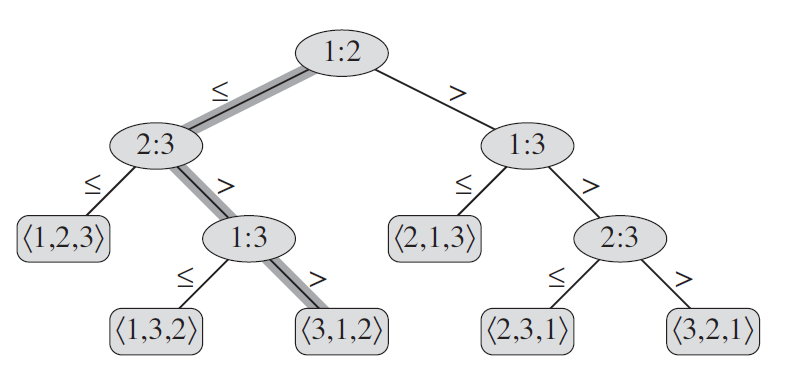
\includegraphics[scale=0.35]{img/alberodidecisione.png}
\end{center}

\section{Altri algoritmi}
\subsection{\href{http://www.cs.miami.edu/home/burt/learning/Csc517.101/workbook/countingsort.html}{\texttt{COUNTING-SORT}}}
Suppone che ciascuno degli elementi di input sia un numero intero compreso tra 0 e k. Quando $k =O(n)$,
l’ordinamento viene effettuato nel tempo $\Theta(n)$.
Per ogni elemento x di input, determiniamo il numero di elementi minori di x: ad esempio, se ci sono 17
elementi minori di x, allora x è alla posizione 18. Attenzione agli elementi con lo stesso valore!\medskip\\
\texttt{COUNTING-SORT}$(A, B, k)$
\begin{lstlisting}[mathescape=true]
for i = 0 to k
    C[i] = 0
for j = 1 to A.length
    C[A[j]] = C[A[j]] +1
//C[i] ora contiene il numero di elementi uguali a i
for i = 1 to k
    C[i] = C[i] + C[i-1]
//C[i] contiene il nuemro di elementi $\leq$ i
for j = A.length downto 1
    B[C[A[j]]] = A[j]
    C[A[j]] = C[A[j]]-1
\end{lstlisting}
riga 1. Dopo aver creato l’array C, inizializza tutti i valori a 0; riga 4.Conteggio del numero di elementi; riga 10. C contiene gli elementi di input ripetuti una sola volta\medskip\\
A[1..n] input;\\ B[1..n] array ordinato;\\ C[0..k] memoria temporanea

\subsection{\texttt{RADIX-SORT}}
È l’algoritmo usato per ordinare le schede perforate. Ordina
prima in base alla cifra meno significativa, combina le schede in
un unico mazzo, poi riordina in base alla seconda cifra meno
significativa e così via.
Se abbiamo un numero di cifre d, occorreranno d passaggi
attraverso il mazzo per completare l’ordinamento.
\begin{center}
      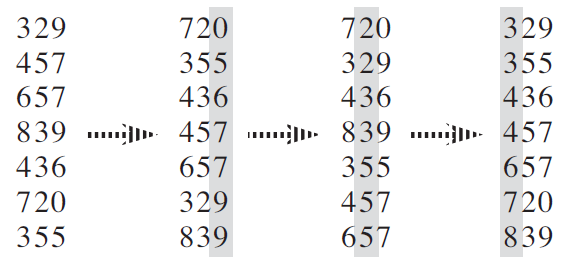
\includegraphics[scale=0.4]{img/radixsort.png}
\end{center}
\texttt{RADIX-SORT}$(A, d)$
\begin{lstlisting}
for i = 1 to d
    do usa ordinamento stabile per ordinare array A su cifra i
\end{lstlisting}
L’algoritmo ordina nel tempo $\Theta(d(n+k))$ dove $n$ è il numero degli input, d è il numero di cifre e k il valore
massimo che una cifra può assumere.
L’algoritmo ordina nel tempo $\Theta((b/r)(n+2^r))$ dove b è il numero di bit e $r \leq b$

\section{Mediane e statistiche d'ordine}
L’i-esima \textbf{statistica d’ordine} di un insieme di $n$ elementi è l’i-esimo numero più piccolo.
Il \textbf{minimo} è la prima statistica d’ordine, il \textbf{massimo} l’n-esima.
La \textbf{mediana} è il “punto di mezzo” dell’insieme. Se n è dispari essa è unica, se $n$ è pari avremo una \textbf{mediana
inferiore} $i = \lfloor(n + 1)/2\rfloor$ e una \textbf{mediana superiore} $i = \lceil(n + 1)/2\rceil$.

Per determinare il minimo (o il massimo) di un insieme di n elementi, servono al massimo $n-1$ confronti.
Per trovare minimo e massimo simultaneamente, sono sufficienti al massimo $3\lfloor \frac{n}{2} \rfloor$ confronti: bisogna
conservare gli ultimi elementi minimo e massimo che si sono trovati. Confrontiamo due elementi di input
l’uno con l’altro; il più piccolo lo confrontiamo col minimo corrente e il più grande con il massimo corrente.
Se $n$ è dispari, assegniamo al minimo e al massimo il valore del primo input, se $n$ è pari confrontiamoi primi
due elementi e diventeranno uno il minimo e uno il massimo.
Se $n$ è dispari svolgiamo $3\lfloor \frac{n}{2} \rfloor$ confronti, se n è pari invece $3 \frac{n}{2}-2$.

\section{\texttt{RANDOMIZED-SELECT}}
\texttt{RANDOMIZED-SELECT} è un algoritmo divide et impera modellato sull’algoritmo \texttt{QUICK-SORT}. Opera solo su
un lato della partizione ed è randomizzato. Il tempo di esecuzione atteso è $\Theta(n)$, mentre nel caso peggiore $\Theta(n^2).$\medskip\\
\texttt{RANDOMIZED-SELECT}$(A, p, r, i)$
\begin{lstlisting}[mathescape=true]
if p = r
    return A[p]
q = $\texttt{RANDOMIZED-PARTITION}(A, p, r)$
k = q - p + 1
if i = k //il valore del pivot e' la soluzione
    return A[q]
else if i < k
    return $\texttt{RANDOMIZED-SELECT}(A, p, q-1, i)$
else return $\texttt{RANDOMIZED-SELECT}(A, q+1, r, i-k)$
\end{lstlisting}
riga 6. A[q] è il pivot\\
riga 8. opera ricorsivamente sul lato sx della partizione\\
riga 9. opera ricorsivamente sul lato dx della partizione\medskip\\
Alla fine di \texttt{PARTITION} abbiamo il pivot al centro, alla sua sx gli elementi (non necessariamente ordinati) più piccoli, a
dx quelli (non necessariamente ordinati) più grandi.

\section{Insiemi dinamici}
Gli insiemi manipolati dagli algoritmi possono cambiare nel tempo: sono detti \textbf{dinamici}.
Gli algoritmi possono richiedere vari tipi di operazioni da svolgere sugli insiemi. Un insieme dinamico che
supporta queste operazioni è detto \textbf{dizionario}.
In un insieme dinamico, un elemento è rappresentato di un oggetto i cui campi possono essere manipolati
se vi è un puntatore all’oggetto.
Per alcuni tipi di insiemi dinamici si suppone che uno dei campi dell’oggetto sia un campo chiave di
identificazione. L’oggetto può contenere dati satelliti.

\subsection{Operazioni sugli insiemi dinamici}
Le operazioni si dividono in \textbf{query} (interrogazioni, che restituiscono informazioni sull’insieme) e \textbf{operazioni di modifica}.
Esse sono:
\begin{itemize}[leftmargin=*, noitemsep]
  \item \texttt{SEARCH}$(S, k)$
  \item \texttt{INSERT}$(S, x)$
  \item \texttt{DELETE}$(S, x)$
  \item \texttt{MINIMUM}$(S)$
  \item \texttt{MAXIMUM}$(S)$
  \item \texttt{SUCCESSOR}$(S, x)$
  \item \texttt{PREDECESSOR}$(S, x)$.
\end{itemize}

\section{Strutture dati elementari}
Stack e code - Sono insiemi dinamici dove l’elemento che viene rimosso dall’operazione delete è
predeterminato. Lo stack (pila) implementa lo schema LIFO, la coda FIFO.

\subsection{Stack}
\begin{itemize}[leftmargin=*, noitemsep]
  \item \texttt{INSERT} = \texttt{\textbf{PUSH}}
  \item \texttt{DELETE} = \texttt{\textbf{POP}}
  \item top[S] = indice dell’ultimo elemento inserito
\end{itemize}
Se si tenta di estarre un elemento da uno stack vuoto (top[S] = 0), si ha un \textbf{underflow} dello stack; se top[S]
supera n, si ha un \textbf{overflow}.\medskip\\
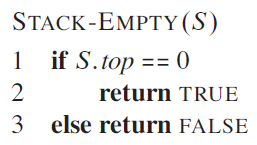
\includegraphics[scale=0.35]{img/stack1.png}\ \ \ \ \
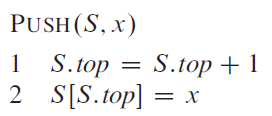
\includegraphics[scale=0.35]{img/stack2.png}\ \ \ \ \
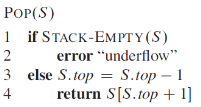
\includegraphics[scale=0.7]{img/stack3.png}

\subsection{Code}
\begin{itemize}[leftmargin=*, noitemsep]
  \item \texttt{INSERT} = \texttt{\textbf{ENQUEUE}} \emph{/enkju:/}
  \item \texttt{DELETE} = \texttt{\textbf{DEQUEUE}} \emph{/dekju:/}
  \item head[Q] = inizio della coda (testa)
  \item tail[Q] = fine della coda (coda)
\end{itemize}
Se head[Q] = tail[Q] la coda è vuota. All’inizio head[Q] = tail[Q] = 1. Se si tenta di rimuovere un elemento da una coda vuota, avremo un underflow; se head[Q] = tail[Q] +1, la coda è piena e il tentetivo di inserire un elemento provocherà un overflow.\medskip\\
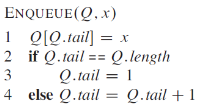
\includegraphics[scale=0.7]{img/coda1.png}\ \ \ \ \ \ \ \ \ \ \ \ \ \ \
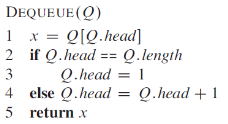
\includegraphics[scale=0.7]{img/coda2.png}

\subsection{Liste concatenate}
È una struttura dati i cui oggetti sono disposti in ordine lineare (ordine determinato da un puntatore in ogni oggetto).

In una \textbf{lista doppiamente concatenata} l’oggetto ha un campo chiave \textbf{key} e due campi puntatori \textbf{next} e \textbf{prev}.
L’oggetto può anche contenere dati satelliti.\\
• head[L] (testa) : prev[x] = NIL\\
• head[L] = NIL – lista vuota\medskip\\
Una \textbf{lista singolarmente concatenata} ha solo il puntatore next.\\
Una lista può essere non ordinata.\\
In una\textbf{lista circolare}, prev[head[L]] == tail[L] e next[tail[L]] == head[L].
\medskip\medskip\medskip
\begin{center}
      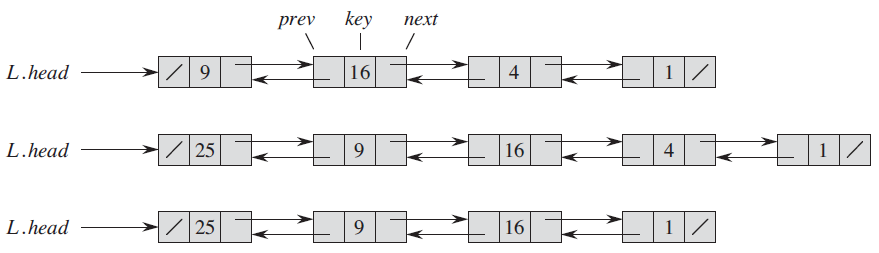
\includegraphics[scale=0.35]{img/listaconcatenata1.png}\medskip\medskip\medskip\\
      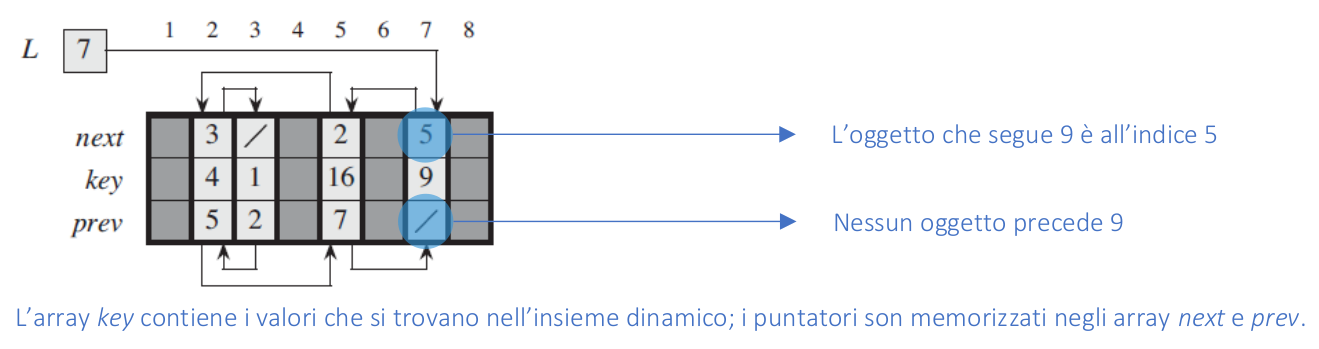
\includegraphics[scale=0.3]{img/listaconcatenata2.png}\medskip\medskip\medskip
\end{center}
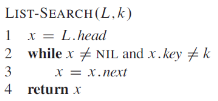
\includegraphics[scale=0.7]{img/listsearch.png}\ \ \ \
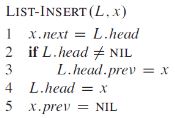
\includegraphics[scale=0.7]{img/listinsert.png}\ \ \ \
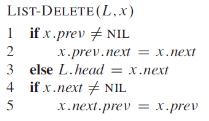
\includegraphics[scale=0.7]{img/listdelete.png}\medskip\medskip\medskip\medskip\\
%
Una \textbf{sentinella} è un oggetto fittizio che consente di semplificare le condizioni al contorno.
Se sostiuiamo la sentinella nil[L] ad ogni riferimento a NIL, avremo una lista doppiamente concatenata con
sentinella.
Una lista vuota è formata solo da una sentinella.
Le sentinelle vanno usate con attenzione: talvolta possono essere uno spreco di memoria.

\subsection{Allocare e liberare gli oggetti}
Supponiamo che gli array abbiano lunghezza $m$ e contengano n elementi. Se $n < m$, $m-n$ elementi sono liberi
e possono essere utilizzati per rappresentare gli elementi da inserire in futuro. Manteniamo gli oggetti liberi
nella lista concatenata \textbf{free list} (è uno stack). La testa della free list è nella variabile globale \textbf{free}. Quando
l’insieme dinamico rappresentato dalla lista concatenata L non è vuoto, L può essere intrecciato alla free list.
Ogni oggetto nella rappresentazione può trovarsi in una sola delle due liste.\medskip\\
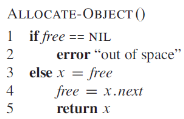
\includegraphics[scale=0.8]{img/allocare.png}\ \ \ \ \ \ \ \ \ \ \ \ \ \ \
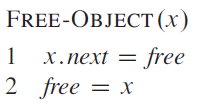
\includegraphics[scale=0.4]{img/deallocare.png}\medskip\\
Le due procedure sono eseguite nel tempo $O(1)$.

\subsection{Alberi binari}
Utilizziamo i campi $p$, $left$ e $rigth$ per memorizzare rispettivamente padre, figlio sx e figlio dx. L’attributo
root[T] punta alla radice dell’albero; se root[T] = NIL allora l’albero è vuoto.

\subsubsection{Rappresentazione figlio-sinistro fratello-destro}
\begin{center}
      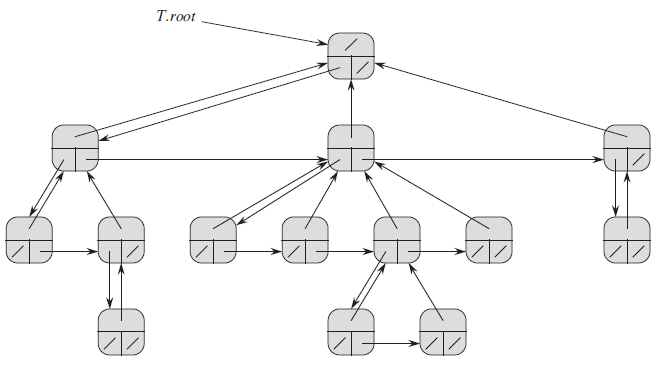
\includegraphics[scale=.4]{img/figliosxfratellodx.png}
\end{center}
Prevede che un nodo x abbia solo due puntatori:\\
- left-child[x] punta al figlio di x più a sx\\
- right-sibling[x] punta al fratello di x immediatamente a destra

\subsection{Tabella a indirizzamento diretto}
L’indirizzamento diretto funziona bene quando l’universo U delle chiavi è ragionevolmente
piccolo.
Supponiamo che un’applicazione abbia bisogno di un insieme dinamico in cui ogni
elemento ha una chiave estratta da U e che due elementi non possano avere la stessa
chiave. Possiamo usare un array o tabella a indirizzamento diretto $T[0 .. m-1]$, dove ogni
\textbf{slot} corrisponde a una chiave in U.
\begin{center}
      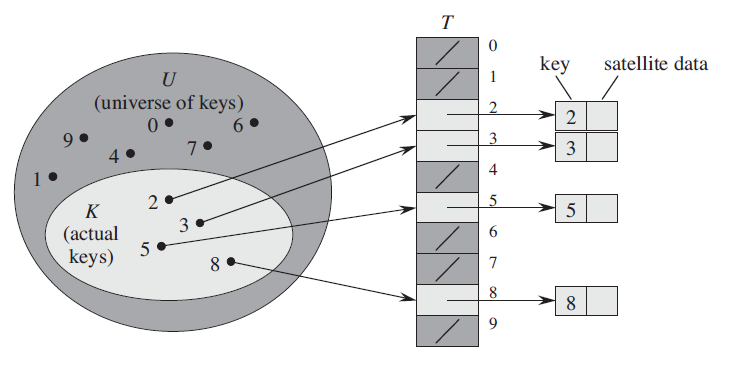
\includegraphics[scale=0.4]{img/indirizzamentodiretto.png}
\end{center}

\subsubsection{Operazioni del dizionario}
\begin{center}
      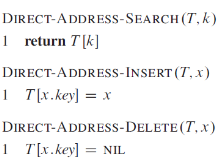
\includegraphics[scale=0.7]{img/dizionario.png}
\end{center}
In alcune applicazioni, possiamo risparmiare spazio memorizzando l’oggetto nello slot stesso (e non in un
elemento esterno alla tabella con un puntatore dalla tabella all’oggetto).

\subsection{Tabelle hash}
Quando l’insieme K delle chiavi è molto più piccolo di U, una tabella hash richiede molto meno spazio di una
tabella a indirizzamento diretto (lo spazio sarà $\Theta(|K|))$.
Con l’indirizzamento diretto, un elemento con chiave $k$ è memorizzato nello slot $k$; con \textbf{l’hashing} è
memorizzato nello slot $h(k)$; ovvero utilizziamo una \textbf{funzione hash} per calcolare lo slot della chiave.
h associa U agli slot di una \textbf{tabella hash}.
\[h: U \rightarrow {0, 1, ..., m - 1}\]
$h(k)$ è il valore hash della chiave k.

\subsubsection{Risoluzione delle collisioni mediante concatenamento}
C’è un problema: due chiavi possono essere associate allo stesso slot (\textbf{collisione}). Evitare le collisioni è
impossibile.
Nel \textbf{concatenamento} poniamo tutti gli elementi che sono associati allo stesso slot in una lista concatenata. Lo
slot in questione contiene un puntatore alla testa della lista di tutti gli elementi che corrispondono allo slot;
se questi elementi non esistono, lo slot conterrà NIL.

\subsubsection{Operazioni del dizionario}
\begin{center}
      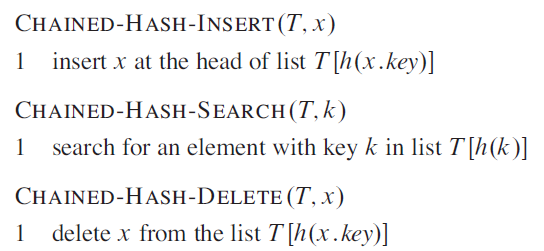
\includegraphics[scale=0.35]{img/dizionario2.png}
\end{center}
\subsubsection{Analisi dell’hashing con concatenamento}
Dati una tabella hash $T$ con $m$ slot in cui sono memorizzati $n$ elementi, definiamo fattore di carico $\alpha$ della
tabella $T$ il rapporto $\frac{n}{m}$ (numero medio di elementi memorizzati in una catena).
Se tutte le n chiavi sono associate allo stesso slot (caso peggiore), il tempo di esecuzione della ricerca sarà
$\Theta(n)$.

\paragraph{Hashing uniforme semplice} se qualsiasi elemento ha le stesse probabilità di essere associato a uno qualsiasi
degli slot, indipendentemente dallo slot cui sarà associato qualsiasi altro elemento.
\begin{itemize}
  \item (nell’ipotesi di hashing uniforme semplice) in una tabella le cui collisioni sono risolte con concatenamento,
  una ricerca senza successo richiede un tempo atteso $\Theta(1+\alpha)$.
  \item  (nell’ipotesi di hashing uniforme semplice) in una tabella le cui collisioni sono risolte con concatenamento,
  una ricerca con successo richiede in media un tempo $\Theta(1+\alpha)$.
\end{itemize}

\subsubsection{Funzioni hash}
Una buona funzione hash soddisfa l’ipotesi di hashing uniforme semplice. Di solito però non è possibile
verificare questa condizione.
La maggior parte delle funzioni hash suppone che l’universo U delle chiavi sia l’insieme dei numeri naturali:
quindi se le chiavi non sono numeri naturali occorre un metodo per interpretarli come tali.\\
\textbf{Metodo della divisione} - $h(k) = k mod$ m\\
\textbf{Metodo della moltiplicazione} - $h(k) = \lfloor m (k A mod 1)\rfloor$

\section{Alberi binari di ricerca}
Sono strutture dati che supportano molte operazioni sugli insiemi dinamici (\texttt{SEARCH}, \texttt{MAXIMUM}, \texttt{MINIMUM}, \texttt{PREDECESSOR}, \texttt{SUCCESSOR}, \texttt{INSERT}, \texttt{DELETE}). Un albero binario può quindi essere usato sia come dizionario che come coda di priorità.
È organizzato come un albero binario in cui ogni nodo è un oggetto che contiene i campi key, p, left e right
(con il campo root che è la radice dell’albero) il cui \textbf{figlio sx è minore} di esso, mentre il \textbf{figlio dx è maggiore}.

Questa proprietà consente di visualizzare ordinatamente tutte le chiavi con un semplice algoritmo ricorsivo
di \textbf{attraversamento simmetrico} dell’albero (inorder, SND). Possiamo usare un algoritmo di \textbf{attraversamento
anticipato} dell’albero (preorder, NSD) oppure un algoritmo di \textbf{attraversamento posticipato} dell’albero
(postorder, SDN).\medskip\\
%
\begin{tabular}{l l}
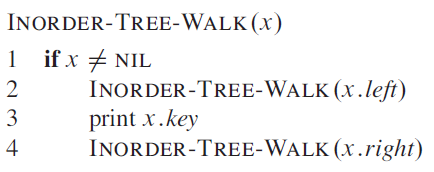
\includegraphics[scale=0.4]{img/tree1.png} \\
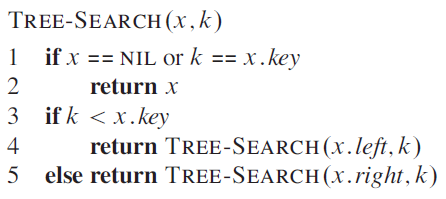
\includegraphics[scale=0.4]{img/tree2.png} & 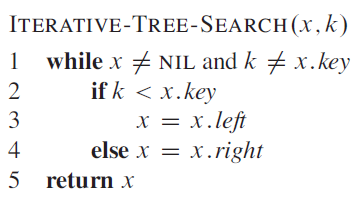
\includegraphics[scale=0.4]{img/tree3.png}\\
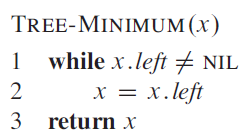
\includegraphics[scale=0.4]{img/tree4.png} & 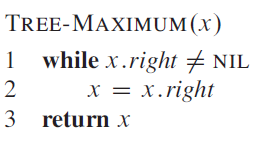
\includegraphics[scale=0.4]{img/tree5.png}\\
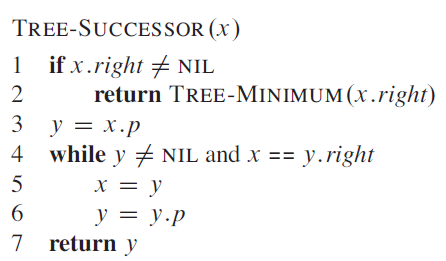
\includegraphics[scale=0.4]{img/tree6.png} & \texttt{TREE-PREDECESSOR}$(x)$ analogo
\end{tabular}
\medskip\\
\begin{tabular}{l l}
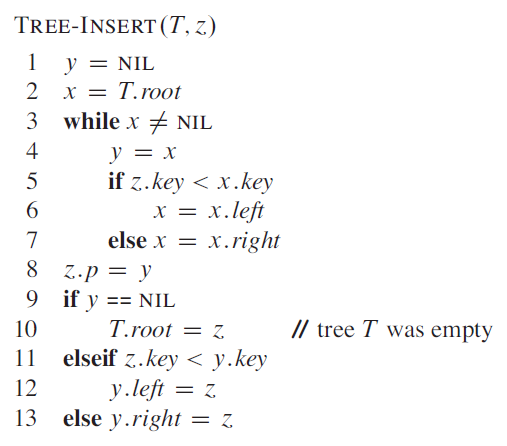
\includegraphics[scale=0.4]{img/tree7.png} \\
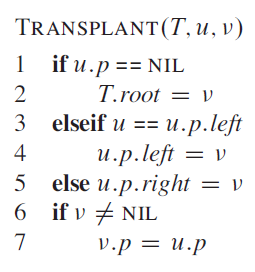
\includegraphics[scale=0.4]{img/tree8.png} & 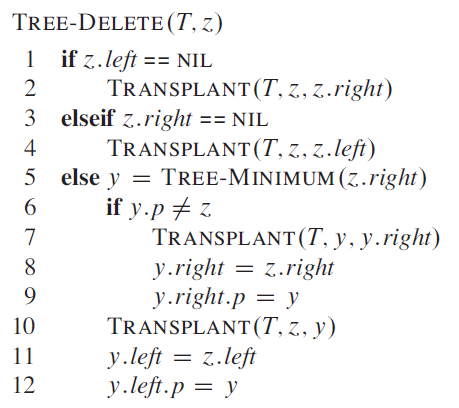
\includegraphics[scale=0.4]{img/tree9.png}\\
\end{tabular}

\section{Riepilogo}
\begin{sideways}
  \begin{tabularx}{550pt}{l|X|c|c|c}
    \multicolumn{2}{c}{\ } & \multicolumn{3}{c}{\textbf{Tempi di esecuzione}}\\
    \hline
    \textbf{Algoritmo} & \textbf{Riassunto} & \textbf{caso migliore} & \textbf{caso peggiore} & \textbf{caso medio}\\
    \hline
    Insertion sort &
    In place. Per un array abbiamo due indici, uno
    punta a l’elemento da controllare, uno a
    quello immediatamente precedente. Se
    l’elemento precedente è più grande, i valori
    vengono scambiati. Confronta l’elemento
    selezionato con tutti i suoi precedenti. &
    $\Theta(n)$ -
    $an+b$ &
    $\Theta(n^2)$ -
    $an^2+bn+c$ &
    $\Theta(n^2)$ \\
    \hline
    Bubble sort &
    Seleziona due elementi e li confronta. Se
    quello precedente è più grande, vengono
    scambiati. Entrambi gli indici aumentano di 1,
    l’algoritmo si ripete. Attraversato tutto
    l’array, si ricomincia. & & \\
    \hline
    Merge (Procedura) &
    Crea due array L e R in cui inserisce la copia
    dei due sottoarray di A più un valore sentinella ($\infty$). Combina (prende i primi
    elemento in L e R e li confronta, inserisce il
    puù grande tra i due nell’array di output.)& &
    $\Theta(n)$
  \end{tabularx}
\end{sideways}

\begin{sideways}
  \begin{tabularx}{550pt}{l|X|c|c|c}
    \multicolumn{2}{c}{\ } & \multicolumn{3}{c}{\textbf{Tempi di esecuzione}}\\
    \hline
    \textbf{Algoritmo} & \textbf{Riassunto} & \textbf{caso migliore} & \textbf{caso peggiore} & \textbf{caso medio}\\
    \hline
    Merge sort &
    Divide et impera. La sequenza di n elementi
    viene divisa in due sottosequenze di n/2
    elementi ciascuna; le due sottosequenze
    vengono risolte in modo ricorsivo tramite
    \texttt{MERGE-SORT}; le sottosequenze ordinate
    vengono unite con \texttt{MERGE} per generare la
    sequenza ordinata (risoluzione del problema) & &
    $\Theta(n \lg n)$ &
    $\Theta(n \lg n)$ \\
    \hline
    Max-heapify (Procedura) &
    Viene determinato il più grande elemento tra
    A[i] e i figli sx e dx. L’indice viene memorizzato
    in massimo. Se A[i] è il più grande, il
    sottoalbero con radice al nodo i è un max-
    heap, altrimenti A[i] viene scambiato con
    A[massimo]. La procedura viene chiamata
    ricorsivamente per tutto l’albero. NB. h è l'altezza del nodo. & &
    $O(\lg n)$ - $O(h)$ \\
  \end{tabularx}
\end{sideways}

\begin{sideways}
  \begin{tabularx}{550pt}{l|X|c|c|c}
    \multicolumn{2}{c}{\ } & \multicolumn{3}{c}{\textbf{Tempi di esecuzione}}\\
    \hline
    \textbf{Algoritmo} & \textbf{Riassunto} & \textbf{caso migliore} & \textbf{caso peggiore} & \textbf{caso medio}\\
    \hline
    Build-max-heap (Procedura) &
    Da un array A[1...n] viene creato un albero
    binario, che viene trasformato in un max-heap
    chiamando la procedura \texttt{MAX-HEAPIFY}. & &
    $O(n)$\\
    \hline
    Heapsort &
    Su un array A[1...n] opera \texttt{BUILD-MAX-
    HEAP}. L’elemento alla radice è dunque il
    maggiore e può essere inserito in A[n]. Viene
    rimosso il nodo n dall’heap (posizionandolo al
    posto della radice). Questo nuovo albero
    viene convertito in un max-heap e si ripete il
    processo. & &
    $O(n \lg n)$ \\
    \hline
    Heap-extract-max &
    La radice viene memorizzata in max.
    Si opera come in \texttt{HEAPSORT} spostando
    l’ultima foglia alla radice e chiamando \texttt{MAX-
    HEAPIFY}. & &
    $O(\lg n)$
  \end{tabularx}
\end{sideways}

\begin{sideways}
  \begin{tabularx}{550pt}{l|X|c|c|c}
    \multicolumn{2}{c}{\ } & \multicolumn{3}{c}{\textbf{Tempi di esecuzione}}\\
    \hline
    \textbf{Algoritmo} & \textbf{Riassunto} & \textbf{caso migliore} & \textbf{caso peggiore} & \textbf{caso medio}\\
    \hline
    Heap-increase-key &
    Ad A[i] viene assegnato il nuovo valore
    (maggiore o uguale al precedente). A[i] viene
    (ripetutamente) confrontato con il padre
    perché potrebbe essere più grande di esso. In
    tal caso le due chiavi vengono tra di loro
    scambiate. & &
    $O(\lg n)$ \\
    \hline
    Max-heap-insert &
    Si aggiunge una foglia al max-heap (con
    chiave $-\infty$). Chiama \texttt{HEAP-INCREASE-KEY}
    per impostare la nuova chiave e mantenere le
    proprietà del max-heap. & &
    $O(\lg n)$ \\
    \hline
    Partition
    (procedura) &
    In place. Seleziona x = A[r] come pivot su cui
    partizionare A[p..r] (elementi minori a sx del
    pivot ed elementi maggiori a dx).
    Viene posto un "muro" tra le posizioni 0 e 1
    dell’array. Si scorre l’array: se l’elemento è
    minore del pivot, viene posto prima del
    muro, altrimenti rimane dopo di esso. Alla
    fine il pivot verrà inserito tra i due gruppi
    dividi dal muro.
    Divide et impera & &
    $\Theta(n)$
  \end{tabularx}
\end{sideways}

\begin{sideways}
  \begin{tabularx}{550pt}{l|X|c|c|c}
    \multicolumn{2}{c}{\ } & \multicolumn{3}{c}{\textbf{Tempi di esecuzione}}\\
    \hline
    \textbf{Algoritmo} & \textbf{Riassunto} & \textbf{caso migliore} & \textbf{caso peggiore} & \textbf{caso medio}\\
    \hline
    Quicksort &
    Divide et impera. In place. Usa ricorsivamente
    \texttt{PARTITION}. & &
    $\Theta(n^2)$ &
    $\Theta(n \lg n)$ - atteso \\
    \hline
    Counting sort &
    Partiamo da un array A. Ogni input è un
    numero intero compreso tra 0 e k. Per ogni
    input x viene determinato il numero di
    elementi minori di x (se vi sono 5 elementi
    minori di x, x è alla posizione 6).
    Creiamo un array C di k+1 elementi (la
    posizione inizia da 0), inizializzati a 0.
    Scorriamo l’array A: ogni volta che
    incontriamo un numero y, incrementiamo di
    1 l’elemento alla posizione y nell’array C
    (stiamo contando per ogni x quanti numeri
    sono uguali a x).
    Ora vogliamo sapere per ogni x quanti numeri
    sono più piccoli o uguali a x: scorriamo l’array
    C e per ogni posizione y sostituiamo la
    somma del valore alla posizione y + il valore
    alla posizione y-1.
    Creiamo un array B della stessa dimensione di
    A. Scorriamo l’array A: inseriamo x nella
    posizione data dall’elemento di C in posizione
    x; decrementiamo di 1 l’elemento in
    questione di C. & &
    $\Theta(k+n)$ &
    $\Theta(k+n)$
  \end{tabularx}
\end{sideways}

\begin{sideways}
  \begin{tabularx}{550pt}{l|X|c|c|c}
    \multicolumn{2}{c}{\ } & \multicolumn{3}{c}{\textbf{Tempi di esecuzione}}\\
    \hline
    \textbf{Algoritmo} & \textbf{Riassunto} & \textbf{caso migliore} & \textbf{caso peggiore} & \textbf{caso medio}\\
    \hline
    Radix sort &
    Ordina tramite un algoritmo stabile ausiliario
    partendo dalla cifra meno significativa a
    quella più significativa. & &
    $\Theta(d(n+k))$ \\
    \hline
    Randomized-select &
    Divide et impera. Opera come quick-sort, ma
    su un solo lato della partizione. & &
    $\Theta(n^2)$ &
    $\Theta(n)$\\
    \hline
    List-search &
    Semplice ricerca lineare che restituisce un
    puntatore all’oggetto. & &
    $\Theta(n)$\\
    \hline
    List-insert &
    Inserisce x davanti alla lista (all’inizio)
    concatenata. & & &
    $O(1)$\\
    \hline
    List-delete &
    Riceve un puntatore a x (dopo aver chiamato
    \texttt{LIST-SEARCH}), elimina x e aggiorna i
    puntatori. & &
    $\Theta(n)$ &
    $O(1)$ \\
    \hline
    Direct-address-search & & & & \multirow{6}{*}{$O(1)$}\\
    Direct-address-insert & & & &\\
    Direct-address-delete & & & &\\
    Chained-hash-insert& & & &\\
    Chained-hash-search& & & &\\
    Chained-hash-delete& & & &\\
    \hline
    Inorder-tree-walk & & & & $\Theta(n) - n nodi$
  \end{tabularx}
\end{sideways}

\begin{sideways}
  \begin{tabularx}{550pt}{l|X|c|c|c}
    \multicolumn{2}{c}{\ } & \multicolumn{3}{c}{\textbf{Tempi di esecuzione}}\\
    \hline
    \textbf{Algoritmo} & \textbf{Riassunto} & \textbf{caso migliore} & \textbf{caso peggiore} & \textbf{caso medio}\\
    \hline
    Tree-search & & & & \multirow{7}{*}{$O(h)$ - h altezza albero}\\
    Tree-minimum & & & & \\
    Tree-maximum & & & & \\
    Tree-successor & & & & \\
    Tree-predecessor & & & & \\
    Tree-insert & & & & \\
    Tree-delete & & & & \\
  \end{tabularx}
\end{sideways}


% TODO: esponenziali, logaritmi, fattoriali .., fibonacci pagina 12 %
% sistemare bubblesort%

%printindex
\end{document}
